\chapter{文献综述}
\section{赤泥的产生和物性}
铝土矿是一种含水氧化铝矿物。典型的含水氧化铝矿物包括三水铝土矿Al(OH)$ _{\mathrm{3}} $,勃姆石$ \gamma $-AlO(OH)和一水硬铝石$\alpha$-AlO(OH)。此外,在铝土矿中一般还含混有针铁矿$\alpha$-FeOOH或赤铁矿Fe$ _{\mathrm{2}} $O$ _{\mathrm{3}} $、少量金红石或锐钛矿TiO$ _{\mathrm{2}} $以及粘土矿高岭石等其他杂质。氧化铝生产工艺主要包括烧结法和拜耳法,但世界上95 \%企业都采用拜耳法工艺\cite{klauber2011bauxite}。图\ref{bayerandsinteringprocess}是氧化铝生产的烧结法和拜耳法的简略工艺流程图。
\begin{figure}[!h]
	\centering
	\vspace{5pt}
	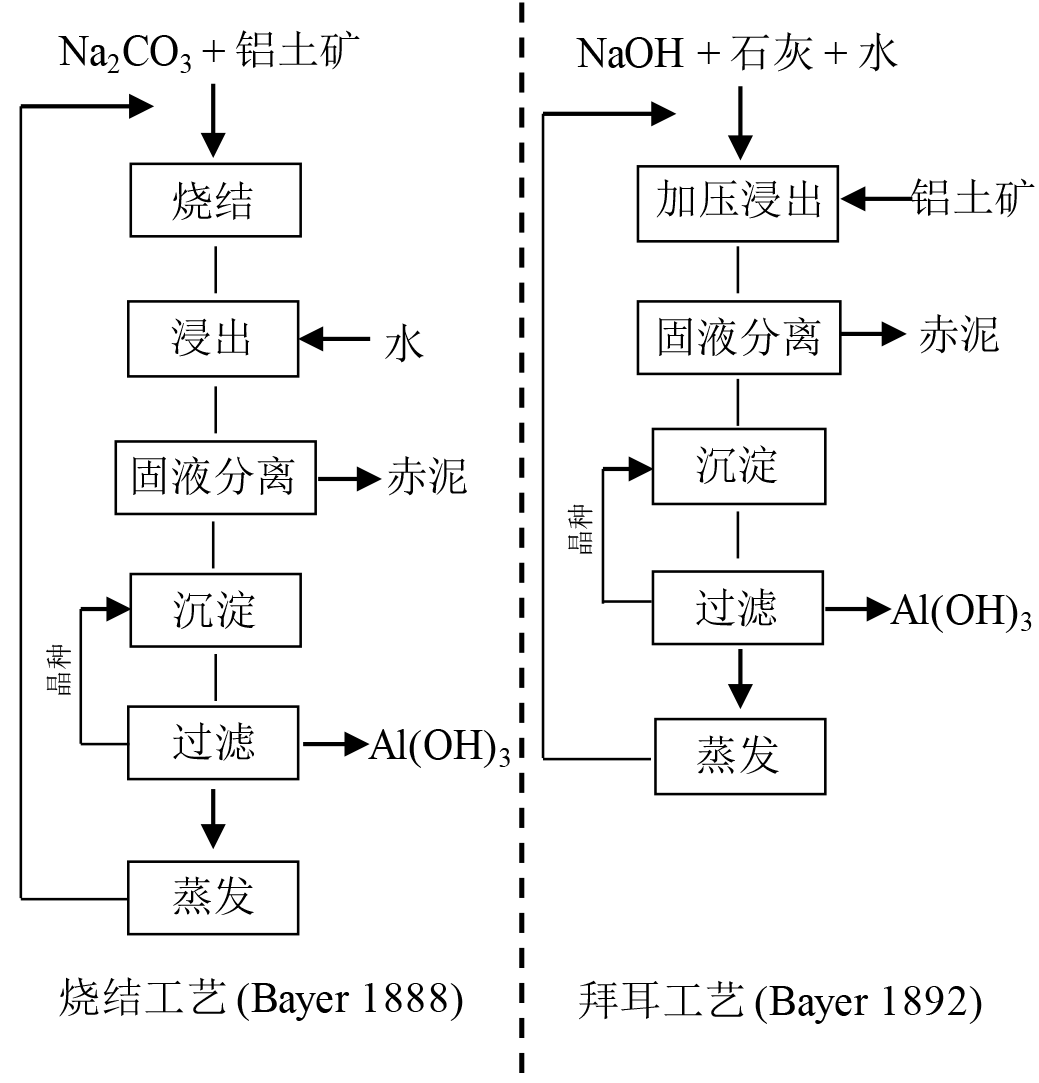
\includegraphics[width=0.65\linewidth]{Figures/c1/bayerandsinteringprocess}
	\caption{拜耳烧结工艺和浸出工艺流程图}\label{bayerandsinteringprocess}
\end{figure}

在拜耳工艺中,不同矿物的工艺参数也不一样。表\ref{processforsanshuilushi}列出了三水铝土矿和一水硬铝石处理工艺部分特点\cite{bauxite1997bishiwen,qing2002yang}。勃姆石或称为一水软铝石的处理工艺参数居于前两种矿物的之间。
\begin{table}[!htbp]
	\centering
	\vspace{-10pt}
	%\setlength{\abovecaptionskip}{18pt plus 0.03ex minus 0.6ex}
	%\setlength{\belowcaptionskip}{12pt plus 0.6ex minus 0.03ex}
	\wu
	\begin{threeparttable}
		\caption{三水铝石和一水硬铝石拜耳处理工艺特点}\label{processforsanshuilushi}
		\begin{tabularx}{\linewidth}{XXX}%p{20pt}指定宽度。
			\toprule[1.5pt]
			参数&一水硬铝石&三水铝石\\\midrule
			溶出温度&245 \textasciitilde{ }280 \textcelsius 或更高&105 \textasciitilde{ }145 \textcelsius\\
			循环母液碱浓度&240 \textasciitilde{ }260 g$ \cdot $L$ ^{\mathrm{-1}} $&140 \textasciitilde{ }180 g$ \cdot $L$ ^{\mathrm{-1}} $\\
			加热蒸汽温度&260 \textcelsius&170 \textasciitilde{ }190 \textcelsius\\
			矿石细磨程度以d$ _{50} $表示&60 \textasciitilde{ }80 μm&0.2 \textasciitilde{ }0.5 mm\\
			溶出反应时间&20 \textasciitilde{ }60 min&2 \textasciitilde{ }5 min\\
			是否需添加石灰&需要&一般不需要\\
			石英是否反应&部分或全部反应&不反应\\
			进料压力&5 \textasciitilde{ }6 MPa&2 \textasciitilde{ }3 MPa\\
			喂料泵型式&隔膜泵&串联离心泵\\
			矿浆预热级数&8 \textasciitilde{ }10 级&2 \textasciitilde{ }3 级\\
			闪蒸级数&7 \textasciitilde{ }9 级&2 \textasciitilde{ }3 级\\
			\bottomrule[1.5pt]
		\end{tabularx}
	\end{threeparttable}
\end{table}

赤泥是一种极细的颗粒,其尺寸一般小于100 μm,比表面积变化在10 \textasciitilde{ }25 m$ \mathrm{^{\mathrm{2}} \cdot g^{\mathrm{-1}}} $\cite{wang2008novel}。图\ref{redmudmicro}a是希腊Agios Nikolaos干赤泥堆置场地\cite{eurare2014}。图\ref{redmudmicro}b是一赤泥微观结构图\cite{zhong2009extraction,liu2007characterization}。赤泥通常是由一系列不同的矿物组成,主要包括赤铁矿Fe$ _{\mathrm{2}} $O$ _{\mathrm{3}} $、针铁矿$ \alpha $-FeOOH、勃姆石$ \gamma $-AlO(OH)、石英SiO$ _{\mathrm{2}} $、方钠石 Na$ _{\mathrm{4}} $Al$ _{\mathrm{3}} $\-Si$ _{\mathrm{3}} $O$ _{\mathrm{12}} $Cl、金红石TiO$ _{\mathrm{2}} $,石膏CaSO$ _{\mathrm{4}} $$ \cdot $H$ _{\mathrm{2}} $O、方解石CaCO$ _{\mathrm{3}} $、水草酸钙CaC$ _{\mathrm{2}} $O$ _{\mathrm{4}} $$ \cdot  $H$ _{\mathrm{2}} $O和三水铝土矿Al(OH)$ _{\mathrm{3}} $。化学分析表明赤泥中主要的元素是Si、Al、Fe、Na、Ca、Ti以及一些微量元素K、Cr、V、Ni、Ba、Cu、Mn、Pb、Zn、Sc、Ga、Ra、U、Th等。在表\ref{redmudscomposition}中,列出了部分世界上不同地方或厂家的赤泥化学成分及其矿物组成\cite{snars2009evaluation,newson2006effect,grafe2011bauxite,paramguru2004trends}。可以发现,赤泥的主要成分是铁氧化物,其次是氧化铝和二氧化硅。
\begin{figure}[!htbp]
	\centering
	\vspace{10pt}
	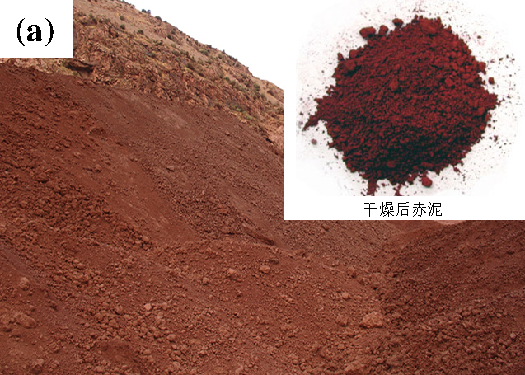
\includegraphics[width=0.45\linewidth]{Figures/c1/Figure3a}\hspace{4pt}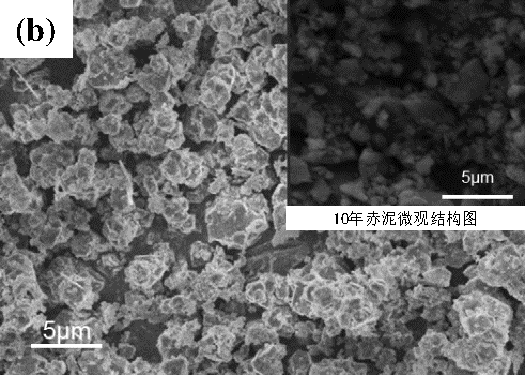
\includegraphics[width=0.45\linewidth]{Figures/c1/Figure3b}
	\caption{拜耳赤泥宏观形貌和微观结构图}\label{redmudmicro}
\end{figure}

赤泥的组成特性除了与铝土矿原料相关外,还与氧化铝的生产工艺十分相关。例如,拜耳赤泥通常没有凝硬性活性。因为在拜耳工艺中,勃姆石或三水铝土矿与热NaOH溶液发生消解,铝以铝酸钠形式浸出,而不会由于固相反应形成活性物质。相反,烧结法赤泥中通常含有$ \beta $-2CaO$ \cdot $SiO$ _{\mathrm{2}} $ 活性物相,而具有凝硬活性。所以烧结法赤泥一般可以直接作为建材原料\cite{liu2009application}。对于高硅低品位铝土矿,通常采用烧结法,若采用拜耳工艺处理低品位铝土矿,则会消耗过多的NaOH反而降低了氧化铝产量\cite{liu2007characterization}。其发生原因可用脱硅产物的生成式\eqref{DSPproduction}来解释。
\begin{equation}\label{DSPproduction}
\begin{split}
& {\rm{1}}{\rm{.7}}\left( {{\rm{A}}{{\rm{l}}_\mathrm{2}}{{\rm{O}}_\mathrm{3}} \cdot {\rm{2}}{\rm{Si}}{{\rm{O}}_{\rm{2}}} \cdot {\rm{2}}{{\rm{H}}_{\rm{2}}}{\rm{O}}} \right) + {\rm{0.6}}{\rm{NaAl}}{\left( {{\rm{OH}}} \right)_{\rm{4}}} + {\rm{3.4}}{\rm{NaOH}} =\\
& {\rm{2}}\left( {{\rm{N}}{{\rm{a}}_{\rm{2}}}{\rm{O}} \cdot {\rm{A}}{{\rm{l}}_{\rm{2}}}{{\rm{O}}_{\rm{3}}} \cdot {\rm{1.7}}{\rm{Si}}{{\rm{O}}_{\rm{2}}} \cdot {\rm{2.6}}{{\rm{H}}_{\rm{2}}}{\rm{O}}} \right) + {\rm{1.1}}{{\rm{H}}_{\rm{2}}}{\rm{O}}
\end{split}
\end{equation}

烧结法和拜耳法工艺中发生的主要反应如下。

铝土矿烧结法:
\begin{equation}
{\rm{N}}{{\rm{a}}_{\rm{2}}}{\rm{C}}{{\rm{O}}_{\rm{3}}}{\rm{ + A}}{{\rm{l}}_{\rm{2}}}{{\rm{O}}_{\rm{3}}} = {\rm{N}}{{\rm{a}}_{\rm{2}}}{\rm{O}} \cdot {\rm{A}}{{\rm{l}}_{\rm{2}}}{{\rm{O}}_{\rm{3}}}{\rm{ + C}}{{\rm{O}}_{\rm{2}}} \rm{(gas)} 
\end{equation}
\begin{equation}
{\rm{2CaO + Si}}{{\rm{O}}_{\rm{2}}} = {\rm{2CaO}} \cdot {\rm{Si}}{{\rm{O}}_{\rm{2}}}\\
\end{equation}
\begin{equation}
{\rm{N}}{{\rm{a}}_{\rm{2}}}{\rm{C}}{{\rm{O}}_{\rm{3}}}{\rm{ + F}}{{\rm{e}}_{\rm{2}}}{{\rm{O}}_{\rm{3}}} = {\rm{N}}{{\rm{a}}_{\rm{2}}}{\rm{O}} \cdot {\rm{F}}{{\rm{e}}_{\rm{2}}}{{\rm{O}}_{\rm{3}}}{\rm{ + C}}{{\rm{O}}_{\rm{2}}} \rm{(gas)} 
\end{equation}
\begin{equation}\label{TiO2+CaO}
{\rm{CaO + Ti}}{{\rm{O}}_{\rm{2}}} = {\rm{CaO}} \cdot {\rm{Ti}}{{\rm{O}}_{\rm{2}}}
\end{equation}

铝土矿拜耳法:

勃姆石与一水硬铝石,
\begin{equation}
\begin{split}
{\rm{AlOOH + NaOH + }}{{\rm{H}}_{\rm{2}}}{\rm{O}} = {\rm{NaAl}}{\left( {{\rm{OH}}} \right)_{\rm{4}}}
\end{split}
\end{equation}

三水铝石,
\begin{equation}\label{bomushi}
\begin{split}
{\rm{Al}}{\left( {{\rm{OH}}} \right)_{\rm{3}}} + {\rm{NaOH} } = {\rm NaAl{\left( {OH} \right)_{\rm{4}}}}
\end{split}
\end{equation}

在我国氧化铝拜耳法生产过程中,通常还加入一定量的石灰以提高铝的溶出率与速度。同时可降低氧化硅的碱耗和消除锐钛矿或金红石不良影响。TiO$ _{\mathrm{2}} $与CaO之间的反应如式\eqref{TiO2+CaO}所示。
\begin{sidewaystable}[!htbp]
	\centering
	\xwu
	\setlength{\belowcaptionskip}{12pt plus 0.6ex minus 0.03ex}
	\begin{threeparttable}
		\caption{世界各地赤泥的主要化学成分和矿相统计表}\label{redmudscomposition}
		\renewcommand\arraystretch{0.85}%设置行距距
		\begin{tabular}{llllllllllll}%p{20pt}指定宽度。
			\toprule[1.5pt]
			化学成分&通常浓度范围(\textit{wt}\%)&巴西&中国 &德国&英国&土耳其&希腊&澳大利亚&印度&牙买加&美国\\
			&&Para state&平果县&Baudart&&Seydisehir&Alhellas&Eurallumia&Damanjodi&Kirkvine&Sherwon\\\midrule
			Fe$ _{\mathrm{2}} $O$ _{\mathrm{3}} $ &6.8 \textasciitilde{ }71.9&45.6&26.9&44.8&36.31&39.84&42.5&35.2&54.8&49.4&50.54\\
			Al$ _{\mathrm{2}} $O$ _{\mathrm{3}} $ &2.1 \textasciitilde{ }33.1&15.1&26.8&16.2&23.43&20.24&15.6&20&14.8&13.2&11.13\\
			TiO$ _{\mathrm{2}} $   &2.5 \textasciitilde{ }22.6&4.29&7.3&12.33&5.97&4.15&5.9&9.2&3.7&7.3&$\circ$\\
			Na$ _{\mathrm{2}} $O  &0.1 \textasciitilde{ }12.4&7.5&$\circ$&4&12.36&9.43&2.4&7.5&4.8&4&9\\
			SiO$ _{\mathrm{2}} $   &0.6 \textasciitilde{ }23.8&15.6&13.1&5.4&18.25&15.27&9.2&11.6&6.4&3&2.56\\
			CaO   &0.6 \textasciitilde{ }47.2&1.16&23.5&5.22&4.38&1.8&19.7&6.7&2.5&9.4&7.73\\
			其他&&10.75&2.4&12.05&0&9.27&4.7&9.8&13&13.7&19.04\\\midrule
			矿相名称&典型化学式(\textit{mol}\%)&巴西&中国 &德国&英国&土耳其&希腊&澳大利亚&印度&新几内亚&意大利\\
			&&Para state&平果县&Boke&&Seydisehir&Alhellas&Eurallumia&Renukoot&Aughinish&Weipa\\\midrule
			非晶相&&$\times$&22&$\times$&38.2&$\times$&$\times$&$\times$&$\times$&$\times$&$\times$\\
			石英&SiO$ _{\mathrm{2}} $&$\bullet$&$\circ$&$\circ$&1.2&$\bullet$&$\circ$&$\circ$&$\circ$&$\bullet$&$\circ$\\
			赤铁矿&$ \alpha $-Fe$ _{\mathrm{2}} $O$ _{\mathrm{3}} $&$\bullet$&19&$\bullet$&13.5&$\bullet$&$\bullet$&29&22.2&$\bullet$&$\bullet$\\
			针铁矿& $ \alpha $-FeO(OH)&$\bullet$&$\circ$&$\bullet$&21.8&$\bullet$&$\circ$&$\circ$&10.9&$\bullet$&$\bullet$\\
			磁铁矿& Fe$ _{\mathrm{3}} $O$ _{\mathrm{4}} $&$\circ$&$\circ$&$\circ$&$\circ$&$\circ$&$\bullet$&$\circ$&$\circ$&$\circ$&$\circ$\\
			钛铁矿& FeTiO$ _{\mathrm{3}} $&$\circ$&10&$\circ$&$\circ$&$\circ$&$\circ$&$\circ$&$\circ$&$\circ$&$\circ$\\
			金红石& TiO$ _{\mathrm{2}} $&$\circ$&3&$\circ$&4.6&$\bullet$&$\bullet$&$\circ$&1.8&$\bullet$&$\circ$\\
			锐钛矿&TiO$ _{\mathrm{2}} $&$\circ$&$\circ$&$\bullet$&$\circ$&$\circ$&$\circ$&5&3.8&$\circ$&$\bullet$\\
			钙钛矿& CaTiO$ _{\mathrm{3}} $&$\circ$&$\circ$&$\circ$&$\circ$&$\circ$&$\bullet$&$\circ$&1.1&$\bullet$&$\circ$\\
			方解石& CaCO$ _{\mathrm{3}} $&$\bullet$&$\circ$&$\bullet$&0.7&$\circ$&$\bullet$&$\circ$&1&$\circ$&$\circ$\\
			三水铝矿& Al(OH)$ _{\mathrm{3}} $&$\bullet$&$\circ$&$\bullet$&$\circ$&$\bullet$&$\circ$&$\circ$&3&$\bullet$&$\circ$\\
			硬水铝石& $ \alpha $-AlO(OH)&$\circ$&$\circ$&$\circ$&$\circ$&$\circ$&$\circ$&5&0.6&$\circ$&$\circ$\\
			软水铝石& $ \gamma $-AlO(OH)&$\circ$&$\circ$&$\circ$&$\circ$&$\circ$&$\circ$&6&1&$\circ$&$\circ$\\
			硅酸钙& CaSiO$ _{\mathrm{4}} $&$\circ$&$\circ$&$\circ$&$\circ$&$\circ$&$\circ$&$\circ$&$\circ$&$\circ$&$\circ$\\
			伊毛缟石& Al$ _{\mathrm{2}} $SiO$ _{\mathrm{3}} $(OH)$ _{\mathrm{4}} $&$\circ$&32&$\circ$&$\circ$&$\circ$&$\circ$&$\circ$&$\circ$&$\circ$&$\circ$\\
			方钠石& Na$ _{\mathrm{4}} $(Si$ _{\mathrm{3}} $Al$ _{\mathrm{3}} $)O$ _{\mathrm{12}} $Cl&$\circ$&$\circ$&$\circ$&17.5&$\circ$&$\circ$&16&3.7&$\circ$&$\circ$\\
			水铝钙石& Ca$ _{\mathrm{4}} $Al(OH)$ _{\mathrm{12}} $$ \cdot $CO$ _{\mathrm{3}} $&$\circ$&$\circ$&$\circ$&$\circ$&$\circ$&$\circ$&$\circ$&$\circ$&$\circ$&$\circ$\\
			钙霞石& Na$ _{\mathrm{6}} $(Al$ _{\mathrm{6}} $Si$ _{\mathrm{6}} $O$ _{\mathrm{24}} $)$ \cdot $2CaCO$ _{\mathrm{3}} $&$\circ$&$\circ$&$\circ$&$\circ$&$\circ$&$\circ$&33&4.7&$\circ$&$\circ$\\
			白云石& Al$ _{\mathrm{2}} $(Si$ _{\mathrm{3}} $Al)O$ _{\mathrm{10}} $(OH,F)$ _{\mathrm{2}} $&$\circ$&$\circ$&$\circ$&2.4&$\circ$&$\circ$&$\circ$&$\circ$&$\circ$&$\circ$\\
			高岭石& Al$ _{\mathrm{2}} $Si$ _{\mathrm{2}} $O$ _{\mathrm{5}} $(OH)$ _{\mathrm{4}} $&$\circ$&$\circ$&$\circ$&$\circ$&$\circ$&$\circ$&$\circ$&$\circ$&$\circ$&$\circ$\\
			伊利石&&$\circ$&$\circ$&$\circ$&$\circ$&$\circ$&$\circ$&$\circ$&$\circ$&$\circ$&$\circ$\\\bottomrule[1.5pt]
		\end{tabular}
		$\circ$:没找到;$ \bullet $:存在;$ \times $:没有检测到;
		伊利石分子式:(K,H$ _{\mathrm{3}} $O)(Al,Mg,Fe)$ _{\mathrm{2}} $(Si,Al)$ _{\mathrm{4}} $O$ _{\mathrm{10}} $[(OH)$ _{\mathrm{2}} $(H$ _{\mathrm{2}} $O)]
		\end{threeparttable}
\end{sidewaystable}

拜耳工艺中NaOH的使用导致赤泥一般具有强碱性与腐蚀性,这种特性并不利于赤泥的再利用。有研究人员曾指出,用1000:1的液固比水洗赤泥,洗涤液的pH值仍然较高,其值甚至可高达10.5\cite{samal2015characterization,shao2016preparation}。目前,海水处理、热处理、酸中和处理是降低赤泥碱度的常用方法\cite{wang2008novel}。

\section{赤泥中有价元素的回收}
过去十年中,从赤泥中再回收有价元素已引起研究人员的广泛关注。然而,由于铝土矿和赤泥的矿物成分和质构的差异,相比于铝土矿提铝,从赤泥中较完全的再提铝或其他有价元素就显得不是那么容易了。
\subsection{赤泥中铝钠的回收}	
拜耳赤泥中一般含有2.12 \%  \textasciitilde{ } 33.1 \%的氧化铝\cite{grafe2011bauxite}。最常用的提取方法是湿法冶金的酸浸法。Bosecker\cite{bosecker1986bacterial}用草酸作为浸出剂,发现仅有 \textasciitilde{ }47 \%的氧化铝可被浸出。Vachon\cite{vachon1994chemical}等人尝试过不同酸和不同混合酸浸回收氧化铝,这些酸中包括硫酸、柠檬酸、草酸。当用2:1柠檬酸草酸比的混合酸,在pH 1.5条件下(硫酸调节),赤泥中96 \%的氧化铝可被回收;与用硫酸在pH值为1的铝浸出结果相比,混合有机无机酸更为有效;但由于有机酸的价格,混合酸浸法经济性较差。

Vachon\cite{vachon1994chemical}等人还尝试过用不同微生物酸从赤泥中浸出氧化铝,这些微生物包括污水污泥细菌和\textit{Aspergillus niger、Penicillum notatum、Penicillum simplicissimum、Trichoderma viride}真菌,当赤泥与\textit{P. simplicissimum}真菌生物酸比为1:10 v/v 时,75 \%的氧化铝可被浸出。

水热法处理赤泥后,钠和其他有价元素显示出较好的浸出特性。早在上世纪90年代,Creswell\cite{cresswell1982hydrothermal}和Solymar\cite{solymar1997technical}等人用此方法就获得了较好的钠浸出结果。通常这个方法是将石灰,碳酸钠,赤泥混合物在150 \textasciitilde{ }300 \textcelsius,0.1 \textasciitilde{ }10 MPa,3 \textasciitilde{ }8液固比条件下,反应10 \textasciitilde{ }240 min,把DSP转化为钙铁—钙铝水化石榴石来回收赤泥中的有价元素\cite{cao2013phase,cresswell1982hydrothermal,zhang2011recovery,zhong2009extraction}。唯一需要注意的是这个方法对于贫铁赤泥不太适用,主要是由于低铁导致较低的铁铝类质同象替代率(不利于铝的浸出)和新相NaCaHSiO$ _{\mathrm{4}} $的生成\cite{zhang2011recovery}。关于水热法,Ablamoff\cite{ablamoff1988physical}首先介绍了这个方法是通过水化学破坏方钠石或钙霞石矿物结构回收氧化铝。此外,Li Zhang\cite{zhong2009extraction}等人采用类似水热法的两步法,首先回收氧化铝,然后水解NaCaHSiO$ _{\mathrm{4}} $相回收氧化钠,铝钠回收率可分别达到87.8 \% 和96.4 \%。若把熟石灰与赤泥充分混合消解后,然后再经过水热处理、煅烧、碳酸钠水溶液浸出,铝钠回收率也可分别达到70 \% 和90 \%\cite{liu1997treatment}。

赤泥若首先与一定量的碳酸钙混合,在1400 \textcelsius 熔融一段时间使形成新相(Na,Ca)$ _{\mathrm{2-}\mathit{x}} $(Al,Fe$ ^{\mathrm{3+}} $)$ _{\mathrm{2-}\mathit{x}} $Si$ _{\mathit{x}} $O$ _{\mathrm{4}} $ (0.2 ≤ \textit{x} ≤ 0.5)后,可以得到较高的氧化铝和钠回收率\cite{bruckard2013smelting}。并且Al$ _{\mathrm{2}} $O$ _{\mathrm{3}} $与Na$ _{\mathrm{2}} $CO$ _{\mathrm{3}} $的溶解度随着CaO/SiO$ _{\mathrm{2}} $比值(在0.1 \textasciitilde{ }2范围内)增加而增加。当固液比1:5,浸出温度60 \textcelsius 时,55 \% Al 和90 \% Na可以回收;在相同浸出条件下,固液比1:2,50 \% Al 和 75 \% Na可以回收;一次浸出液再次用于赤泥中有价元素浸出,可以得到含铝130 g$ \cdot $L$ ^{\mathrm{-1}} $和含钠125 g$ \cdot $L$ ^{\mathrm{-1}} $的浸出液。在富铁赤泥添加10 \% \textasciitilde{ }12 \% Na$ _{\mathrm{2}} $O$ \cdot $Fe$ _{\mathrm{2}} $O$ _{\mathrm{3}} $和增加焙烧时间到30 \textasciitilde{ }40 min将十分有利于不溶相3CaO$ \cdot $Al$ _{\mathrm{2}} $O$ _{\mathrm{3}} $,Na$ _{\mathrm{2}} $O$ \cdot $Al$ _{\mathrm{2}} $O$ _{\mathrm{3}} $$ \cdot $2SiO$ _{\mathrm{2}} $ 和4CaO$ \cdot $Al$ _{\mathrm{2}} $O$ _{\mathrm{3}} $$ \cdot $Fe$ _{\mathrm{2}} $O$ _{\mathrm{3}} $发生转变,从而将在一定程度上有利于氧化铝的浸出。此外,烧结温度对铝的浸出也会产生较大影响,因为不同温度伴随着不同的烧结固相反应及产物。新物相形成或旧物相消失的温度点可借助于差热实验反映\cite{zhou2008alumina}。赤泥在800 \textasciitilde{ }1075 \textcelsius 下还原焙烧后,钠铝酸盐和钙硅酸盐中三价铁氧化物可被还原剂还原成磁铁矿或金属铁,氧化铝和氧化铁的回收可通过浸出与磁选(磁场强度48 kA$ \cdot $m$ ^{\mathrm{-1}} $)实现,它们的回收率可分别富集到89.71 \%和60.67 \%\cite{li2009recovery}。苏打—石灰焙烧赤泥,使含铝钠矿物转变为易水解铝酸钠,再采用水浸焙烧产物,75.7 \% Al和80.7 \% Na可被浸出\cite{liu2012experimental}。焙烧过程中相变如下式。
\begin{equation}
\begin{split}
&{\rm{N}}{{\rm{a}}_{\rm{2}}}{\rm{O}} \cdot {\rm{mA}}{{\rm{l}}_{\rm{2}}}{{\rm{O}}_{\rm{3}}} \cdot {\rm{nSi}}{{\rm{O}}_{\rm{2}}} \cdot {\rm{x}}{{\rm{H}}_{\rm{2}}}{\rm{O + 2nCaO + }}\left( {{\rm{m - 1}}} \right){\rm{N}}{{\rm{a}}_{\rm{2}}}{\rm{C}}{{\rm{O}}_{\rm{3}}}{\rm{   = }}\\
&{\rm{mN}}{{\rm{a}}_{\rm{2}}}{\rm{O}} \cdot {\rm{A}}{{\rm{l}}_{\rm{2}}}{{\rm{O}}_{\rm{3}}}{\rm{ + n 2CaO}} \cdot {\rm{Si}}{{\rm{O}}_{\rm{2}}}{\rm{ + x}}{{\rm{H}}_{\rm{2}}}{\rm{O + }}\left( {{\rm{m - 1}}} \right){\rm{C}}{{\rm{O}}_{\rm{2}}}({\rm{gas}})
\end{split}
\end{equation}

需要注意的是氧化硅的热力学活度随着焙烧中氧化钙含量增加而降低,高温时不易形成钠铝硅酸盐相;同时,氧化钙的添加会增加水浸时铝钠溶解度。另外,还原焙烧也可影响铁相平衡系统而有利于铝钠回收。

若在800 \textasciitilde{ }1000 \textcelsius 下焙烧充分混匀后的赤泥、煤、石灰和碳酸钠,然后在65 \textcelsius 水浸一小时,89 \%的铝可被浸出,所得浸出液可直接倒入拜耳工艺流程的母液中。磁选残渣,73 \textasciitilde{ }79 \%的钛富集于非磁性部分,然后可经过硫酸浸出,水解,过滤和焙烧回收钛。在另一方面,磁性部分在1480 \textcelsius 熔融后,可以得到含铁93 \textasciitilde{ }94 \%的生铁块。整个回收工艺流程示意图如图\ref{reducing&magneticseparation}所示\cite{piga1993recovering}。
\begin{figure}[!h]
	\centering
	
	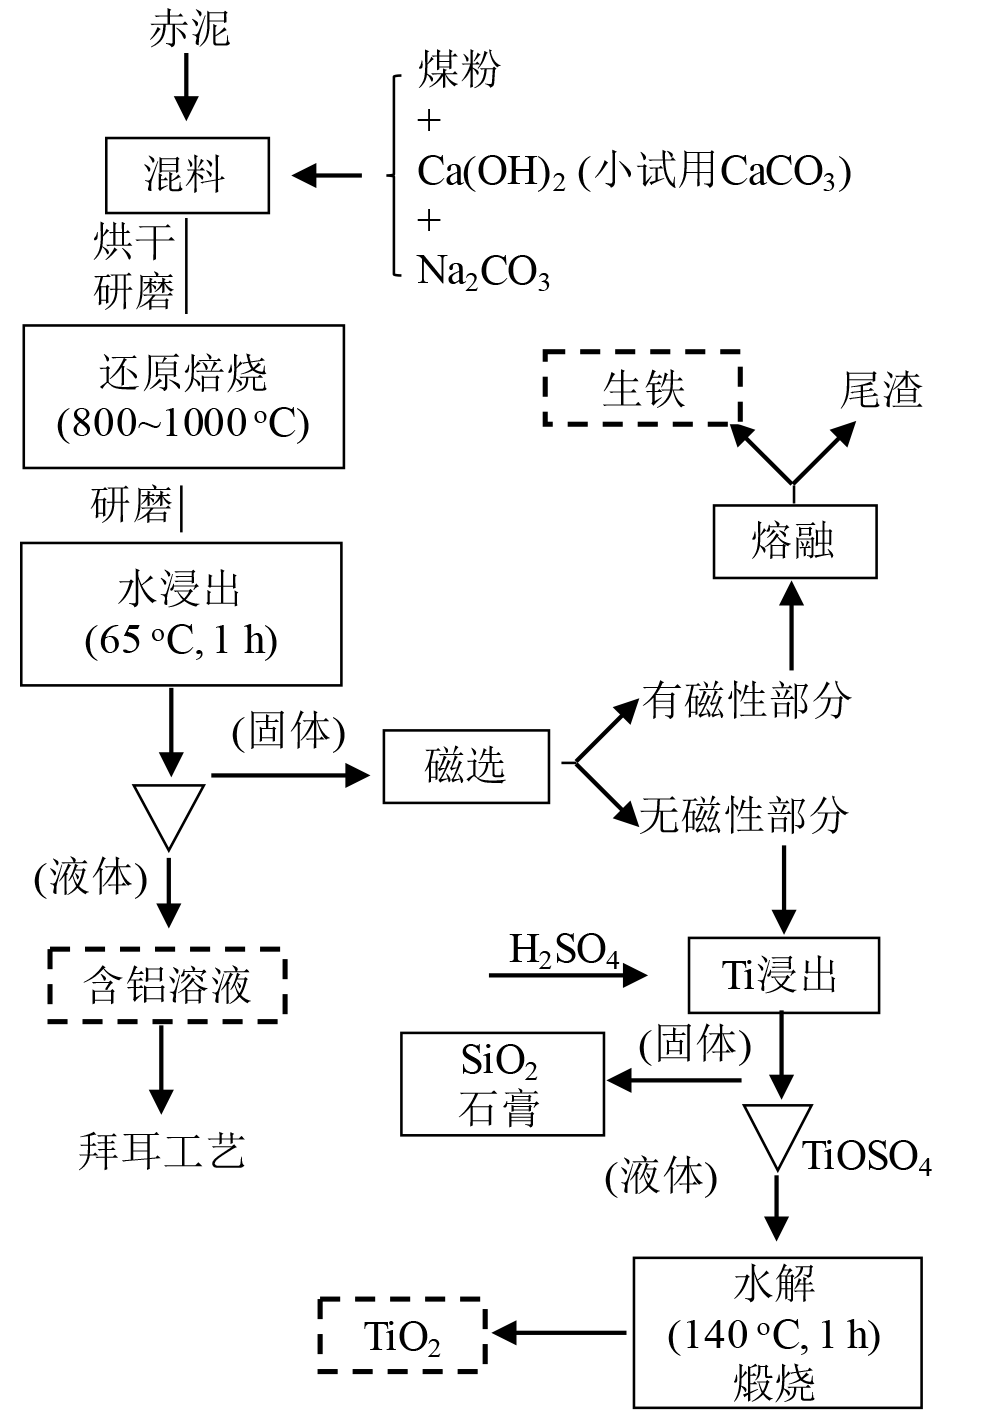
\includegraphics[width=0.65\linewidth]{Figures/c1/Figure4}
	\caption{还原焙烧磁选工艺回收赤泥中铝铁钛流程图}\label{reducing&magneticseparation}
\end{figure}

\begin{figure}[!h]
	\centering
	
	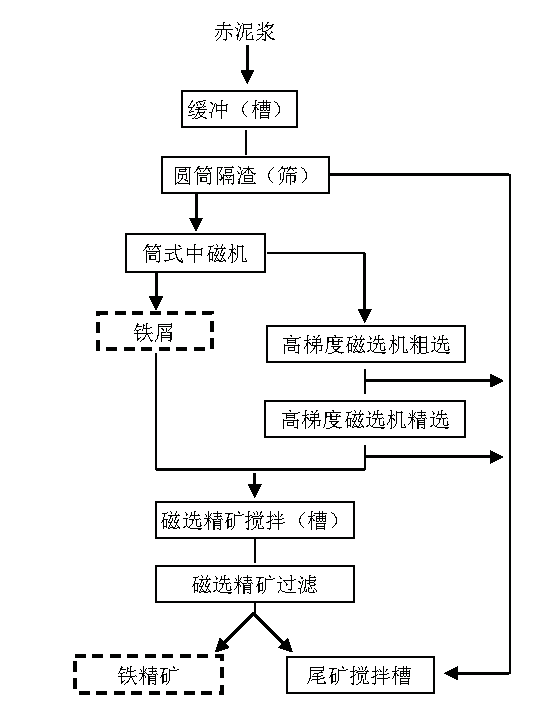
\includegraphics[width=0.65\linewidth]{Figures/c1/Figure5}
	\caption{高梯度磁选法回收赤泥中铁的流程图}\label{highgrademagneticseparation}
\end{figure}
\subsection{赤泥中铁的回收}
如前所述,氧化铁是赤泥中的主要成分,若以三价铁氧化物计,则占赤泥质量分数的6.8 \textit{wt}\% \textasciitilde{ }71.9 \textit{wt}\%,其含量与铝土矿中铁品位直接相关\cite{grafe2011bauxite,jayasankar2012production}。赤泥中铁的回收可由物理方法磁选直接实现。磁选产物可作为炼铁厂烧结原料或作为陶瓷产品的涂料\cite{hammond2013cr,jamieson2006magnetic}。早在1970年,磁选就开始应用于赤泥中铁的回收,只是当时效果较差\cite{liu2015metallurgical}。然而,对经过预处理后的赤泥,若采用脉冲高梯度磁选却显示出较好的分离效果\cite{li2005study}。高梯度超导磁选(HGSMS)相比于普通铁心的电磁铁,由于在悬浮液中可形成更强的磁场,高梯度超导磁选被认为是最有效的分离悬浮液中的细磁性颗粒方式。另一方面,对企业经济成本来说,超导磁体也是可承担的\cite{ohara2001magnetic}。当赤泥颗粒小于100 μm时,铁氧化物形态对磁分离效果也会有影响\cite{li2011feasibility}。HGSMS磁分离结果表明低铁品位赤泥比高铁赤泥磁选效果更好。另外,复杂铁共生和弱磁非磁物料也容易在磁选时同时捕获进入铁精矿,从而降低赤泥铁精矿品位。如果,赤泥先通过筒形中等磁场分离强磁铁部分,尾渣赤泥再经过Slon\textregistered 垂直环状脉冲HGSMS开路粗选和精选回收弱磁铁部分,则可以得到含全铁TFe $ \geq $ 54 \%的铁精矿或28 \% \textasciitilde{ }35 \%的铁回收率\cite{peng2011method}。图\ref{highgrademagneticseparation}是整个铁磁选回收流程示意图。
\begin{figure}[!h]
	\centering
	\setlength{\belowcaptionskip}{6pt plus0.3ex minus 0.06ex}
	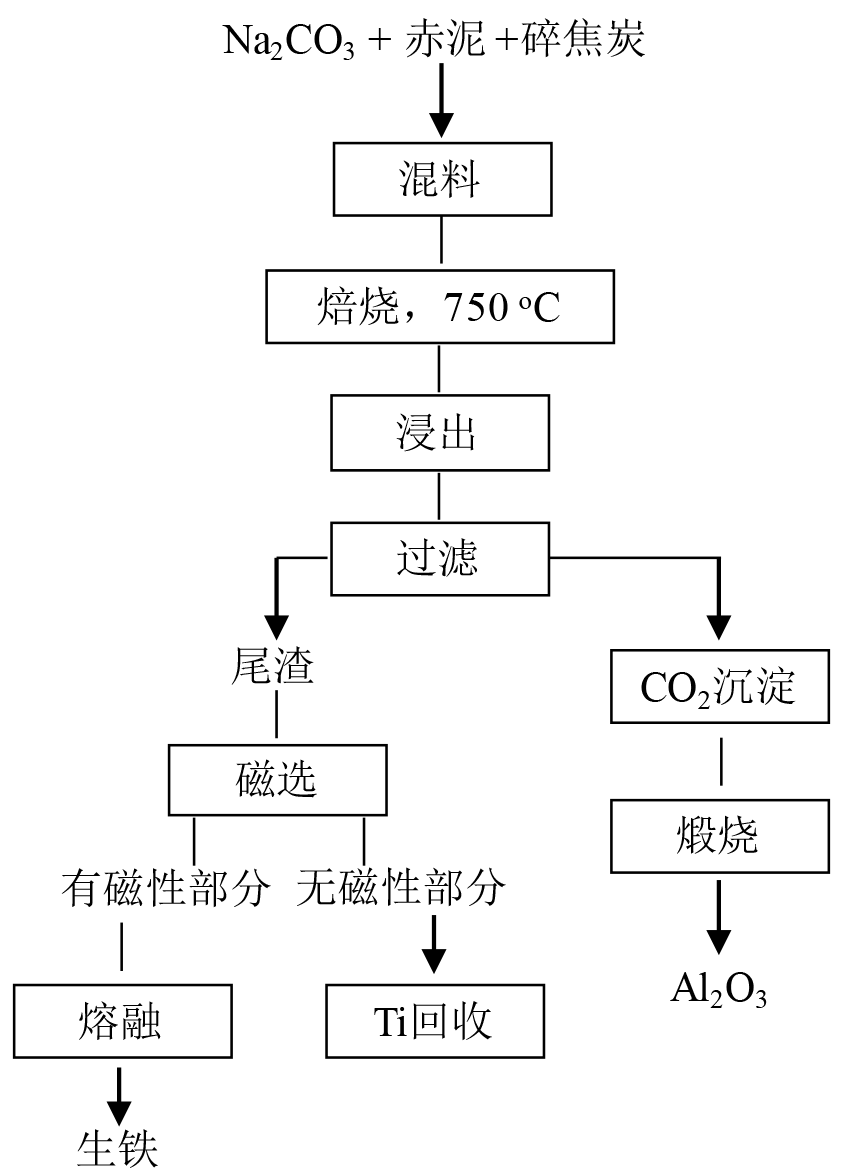
\includegraphics[width=0.65\linewidth]{Figures/c1/Figure6}
	\caption{钠化还原焙烧回收赤泥中铝铁钛流程图}\label{recoveringFe, Al, Ti}
\end{figure}

焙烧和高温熔融还原是从赤泥中回收铁的其他的方法\cite{kumar1998utilization}。简化的典型钠化焙烧和熔融还原法分别如图\ref{recoveringFe, Al, Ti}\cite{kumar1998utilization}和图 \ref{recoveringFe}\cite{zhu2012recovery}所示。在还原熔融赤泥处理方式中,固态还原剂主要包括碳粉\cite{liu2009application,li2009recovery,raspopov2013reduction}、石墨\cite{jayasankar2012production}、烟煤\cite{liu2012experimental} 、煤焦\cite{zhu2012recovery} 、焦炭\cite{rath2013statistical}等。除了还原剂种类对铁还原回收过程的程度和速率影响外,还原剂的反应性和挥发分含量对铁回收也有影响\cite{xiangong1996kinetics}。就煤质而言,煤活性高,灰分少,理论需求量中[(F$ \mathrm{_{c}} $+V$ \mathrm{_{m}} $):(A+W)] (F$ \mathrm{_{c}} $:固定碳含量;V$ \mathrm{_{m}} $:挥发分含量;A:灰分;W: 其他不可燃杂质量)和[(SiO$ _{\mathrm{2}} $+TFe):(Al$ _{\mathrm{2}} $O$ _{\mathrm{3}} $+其他)]比值越大越好\cite{yongkang1995study}。另外,一定量的添加剂如镁盐、钙盐、钠盐及其混合物盐可以提高煤基直接还原富铁赤泥效率。强碱添加剂可以破坏赤泥中复杂铁氧化物结构,同时降低表观活化能而增加还原速率\cite{qiu1996influence}。Jayasankar\cite{jayasankar2012production}等人研究了添加10 \% \textasciitilde{ }16 \%的白云石对铁回收的影响,发现12 \%的添加量可使铁回收达到其最大值约71 \%。硫酸钠和碳酸钠添加量对赤泥中铁磁化率和磁选精矿回收率也有影响。当添加6 \% Na$ _{\mathrm{2}} $SO$ _{\mathrm{4}} $和6 \% Na$ _{\mathrm{2}} $CO$ _{\mathrm{3}} $在1050 \textcelsius 下焙烧60 min后,94.5 \%的铁可被回收\cite{rao2013iron}。若碳粉与赤泥(X$ \mathrm{_{c}} $:X$ \mathrm{_{o}} $=1.6:1)混合物,在碱度值为1.0熔融温度1400 \textcelsius 下,熔融30 min后急冷于液氮中,可得到含96.52 \textit{wt}\% Fe、3.09 \textit{wt}\% C、0.051 \textit{wt}\% Si、0.013 \textit{wt}\% Mn、0.076 \textit{wt}\% P和0.091 \textit{wt}\% S的铁块\cite{guo2013nuggets}。实验结果最终表明:主要影响金属化率是还原温度、时间以及X$ \mathrm{_{c}} $:X$ \mathrm{_{o}} $比值。然而另有研究表明,铸铁在1200 \textasciitilde{ }1500 \textcelsius 时就已与渣完全分离\cite{raspopov2013reduction},与前一结果基本一致。前面所述的焙烧—磁选工艺中,赤泥与添加剂通常各自呈独立的颗粒体。压实含熟石灰的赤泥圆柱生坯在1300 \textcelsius 焙烧30 min后水淬,磁场强度为1 A下磁选可回收了81.40 \%的铁或金属化率为96.98 \%的铁块\cite{liu2009application}。此外,研究人员还对Al、Na回收做了一些研究工作\cite{liu2012experimental},工艺流程类似于图\ref{recoveringFe, Al, Ti}。在苏打—石灰焙烧—浸出工艺后,赤泥浸后渣由磁铁矿Fe$ _{\mathrm{3}} $O$ _{\mathrm{4}} $,铁铝尖晶石Fe(Fe,Al)$ _{\mathrm{2}} $O$ _{\mathrm{4}} $和钛尖晶石TiFe$ _{\mathrm{2}} $O$ _{\mathrm{4}} $组成,然而其51.2 \%铁回收率低于前者的81.40 \%。这可能是由于磁性铁相中还含有其他杂质如斜硅钙石、钙铁铝酸盐和钠铝硅酸盐而导致磁选精矿的含铁量和铁回收率降低。微波辐射也可作为赤泥还原焙烧时的热源\cite{samouhos2013greek}。相比于传统加热方式,微波辐射加热更加洁净和可控,并且理论上不会对电介质产生温度梯度。但是有限的微波源寿命和功率是其最大的缺点。10 \textit{wt}\%焙烧料水溶液在0.3 A磁场强度下湿法磁选后,磁精矿中铁含量可达35.1 \% TFe和69.3 \%的金属化率。相比于传统方法,微波焙烧时间减少了将近40 \%,磁精矿的金属化率也更高。另外,值得一提的是赤泥中的放射性物质在微波焙烧后其放射性低于放射物放射性许可量(1000 Bq$ \cdot $kg$ ^{\mathrm{-1}} $)\cite{samouhos2013greek}。

600 \textcelsius 低温焙烧赤泥后再用6M H$ _{\mathrm{2}} $SO$ _{\mathrm{4}} $酸浸赤泥,可回收97.46 \%的铁,同时64.40 \%的铝可浸出回收,只是其浸出率较铁慢\cite{uzun2007dissolution}。浸出过程中,铁铝的溶解速率满足一级反应机制,也就是$\left[ {{\rm{ - }}\ln \left( {1 - \alpha } \right)} \right] = \mathit{kt}$,此处$ \alpha $铁铝的溶解部分;\textit{t}是时间min;\textit{k}是反应速率常数,min$ ^{\mathrm{-1}} $。草酸也可用于赤泥中铁的浸出\cite{yu2012red}。用1 mol$ \cdot $L$ ^{\mathrm{-1}} $草酸于75 \textcelsius 浸出2 h,96 \%的铁可被浸出。在下一步的水解过程中,UV辐照引起的光催化作用有利于三价铁草酸盐向二价草酸盐($ \beta $-FeC$ _{\mathrm{2}} $O$ _{\mathrm{4}} $$ \cdot $2H$ _{\mathrm{2}} $O)转化。另外,有人对赤泥中Al$ ^{\mathrm{3+}} $、Fe$ ^{\mathrm{3+}} $、Ti$ ^{\mathrm{4+}} $和Na$ ^{\mathrm{+}} $在反萃取相中离子浓度和回收情况基于不同H$ ^{\mathrm{+}} $浓度对阳离子交换膜影响作了研究\cite{cengeloglu2003recovery,ccengelouglu2001recovery},指出H$ ^{\mathrm{+}} $不仅起着离子转运功能,而且平衡输送通量,增加H$ ^{\mathrm{+}} $浓度通常将提高运输效率;在SA$ _{\mathrm{3}} $T膜中,若赤泥溶液稀释两倍后,钠离子的“回收因子”可高达31.90\cite{cengeloglu2003recovery}。湿法浸出法虽然展示出较好的回收效果,但是对目标元素的选择性极低。
\begin{figure}[!h]
	\centering
	%\setlength{\belowcaptionskip}{-10pt plus0.3ex minus 0.06ex}
	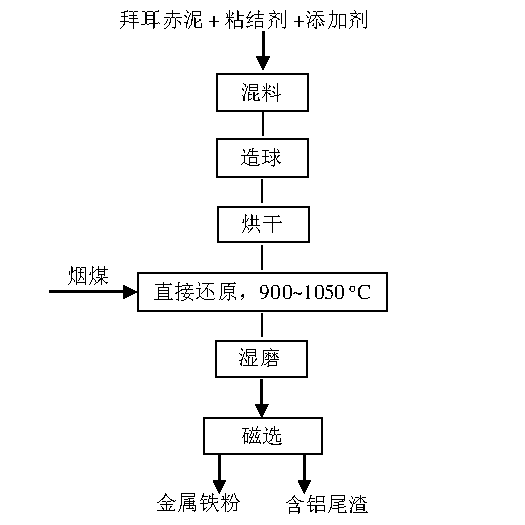
\includegraphics[width=0.65\linewidth]{Figures/c1/Figure7}
	\caption{造球还原焙烧回收赤泥中铁的流程图}\label{recoveringFe}
\end{figure}

在生物浸出铁方面,由于其生态性和低能耗而得到越来越多的关注\cite{laguna2011bioreduction,qu2013bioleaching,eisele2014review}。通常铁矿微生物溶解机制可分为两类。一种是产生的各种有机酸与Fe$ ^{\mathrm{2+}} $和Fe$ ^{\mathrm{3+}} $络合而增加含铁相的溶解浸出性;另一种机制是促进Fe$ ^{\mathrm{3+}} $转变为二价Fe$ ^{\mathrm{2+}} $,这是由于二价铁相对于三价铁复合物有更高的溶解度\cite{eisele2014review}。\textit{Desulfuromonas palmitatis}真菌被认为是可以从铝土矿中溶解部分含铁矿物,例如,非晶形的水铁矿的溶解度可达到95 \%;但该菌相对较高结晶度的针铁矿的溶解度却不超过9 \%;结晶度更高的赤铁矿低于1.2 \%。另外,赤泥液中较高的pH值严格限制了铁氧化物的生物浸出,因此这方面的研究工作较少\cite{papassiopi2010effectiveness}。应用于工业中铁浸出回收工艺,虽然应尽量考虑其经济成本,但同时也应考虑其实用性。
\begin{figure}[!h]
	\centering
	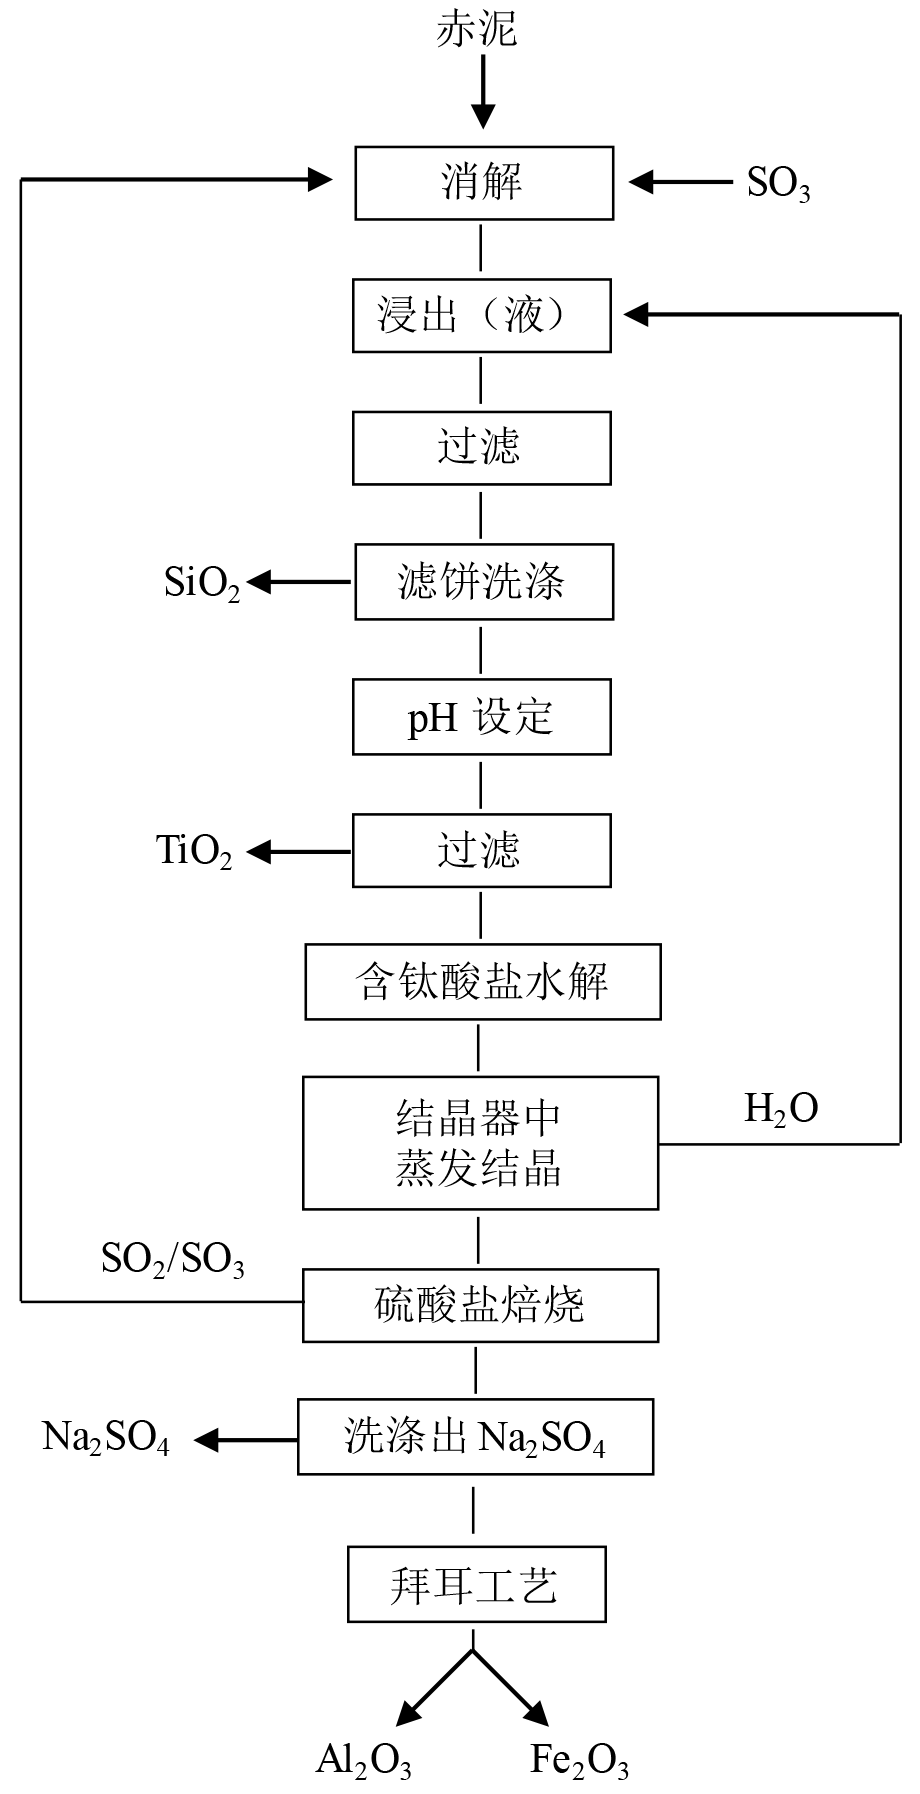
\includegraphics[width=0.65\linewidth]{Figures/c1/Figure8}
	\caption{硫酸或三氧化硫气体回收赤泥中钛钠铝铁流程图}\label{H2SO4orSO3recoveringFe,Na,Al}
\end{figure}

\subsection{赤泥中钛钒的回收}

赤泥中钛元素主要以TiO$ _{\mathrm{2}} $形式存在,它是一种应用广泛的光催化剂和白色涂料。赤泥中金红石或锐钛矿含量一般在2.5 \textit{wt}\% \textasciitilde{ }22.6 \textit{wt}\%之间\cite{grafe2011bauxite},如表\ref{redmudscomposition}所示。用6 N硫酸在60 \textcelsius 和液固比20:1条件下处理赤泥,64.5 \%的钛可被提取出来\cite{agatzini2008titanium,tsakiridis2011synthesis},同时46 \%的铁和约37 \%的铝被同时浸出。Ercag\cite{erccaug1997furnace}等人将赤泥,白云石和焦炭造球后在1100 \textcelsius 焙烧1 h,然后将温度升高到1550 \textcelsius 熔融0.5 h;通过渣铁比重差异,实现生铁分离回收;然后,用30 \% H$ _{\mathrm{2}} $SO$ _{\mathrm{4}} $在90 \textcelsius 洗涤尾渣,用5 \% D2EHPA 煤油萃取稀释浸出液,84.7 \%基于渣重的TiO$ _{\mathrm{2}} $可被回收。Kasliwal和Sai\cite{kasliwal1999enrichment}描述了一个新的方法富集赤泥中的钛。赤泥中的钛首先用盐酸富集到36 \%,随后在1150 \textcelsius 苏打焙烧115 min,水浸除去铝硅二次富集TiO$ _{\mathrm{2}} $到76 \%。除了火法工艺回收钛外,很多研究人员还尝试了用硫酸或SO$ _{\mathrm{3}} $来回收赤泥中的钛。在采用硫酸提钛方面\cite{csayan2000statistical,mehta1951recovery},钛可通过酸浸中产生的RSO$ _{\mathrm{4}} $$ \cdot $Ti(SO$ _{\mathrm{4}} $)$ _{\mathrm{2}} $来回收,此处的R代表Zn、Cu、Mn、Co和Mg。Sayan和Bayramoglu用统计建模法分析了酸浸温度、时间、硫酸pH和液固比对钛的浸出影响。赤泥也可采用硫酸或SO$ _{\mathrm{3}} $在250 \textasciitilde{ }350 \textcelsius 消解成硫酸盐,然后在$ \geq $90 \textcelsius 环境中水解浸出钛\cite{liu2015metallurgical},蒸发过滤后的溶液或与丙酮混合,硫酸钠铝、铁析晶分离出来。然后可通过在900 \textasciitilde{ }1000 \textcelsius 中加热产物使其分解的得到对应的氧化物和SO$ _{\mathrm{3}} $ 与SO$ _{\mathrm{2}} $混合气体。加热分解前,硫酸钠可首先水溶除去,其整个流程如图 \ref{H2SO4orSO3recoveringFe,Na,Al}所示。钛和锆还可通过硫酸浸出和碱熔富集\cite{kasai1994enrichment}。先用稀硫酸于25 \textcelsius 浸出10 min除去赤泥中的方钠石,然后再用0.5 \textasciitilde{ }2 mol$ \cdot $L$ ^{\mathrm{-1}} $ H$ _{\mathrm{2}} $SO$ _{\mathrm{4}} $在120 \textcelsius 中溶解赤铁矿,再经过碱熔过程使氧化硅浸出。经过上述处理后,赤泥中Ti和Zr可分别富集到84 \%和3 \%,图\ref{recoveringTiZr}是其整个工艺流程。在用盐酸浸出回收钛方面,基本上没有什么文献报道。这可能是由于常温下TiO$ _{\mathrm{2}} $在HCl中溶解度较低\cite{kasai1994enrichment,piga1993recovering}。

\begin{figure}[!h]
	\centering
	\vspace{15pt}
	\setlength{\abovecaptionskip}{30pt plus0.3ex minus 0.06ex}
	%\setlength{\belowcaptionskip}{6pt plus0.3ex minus 0.06ex}
	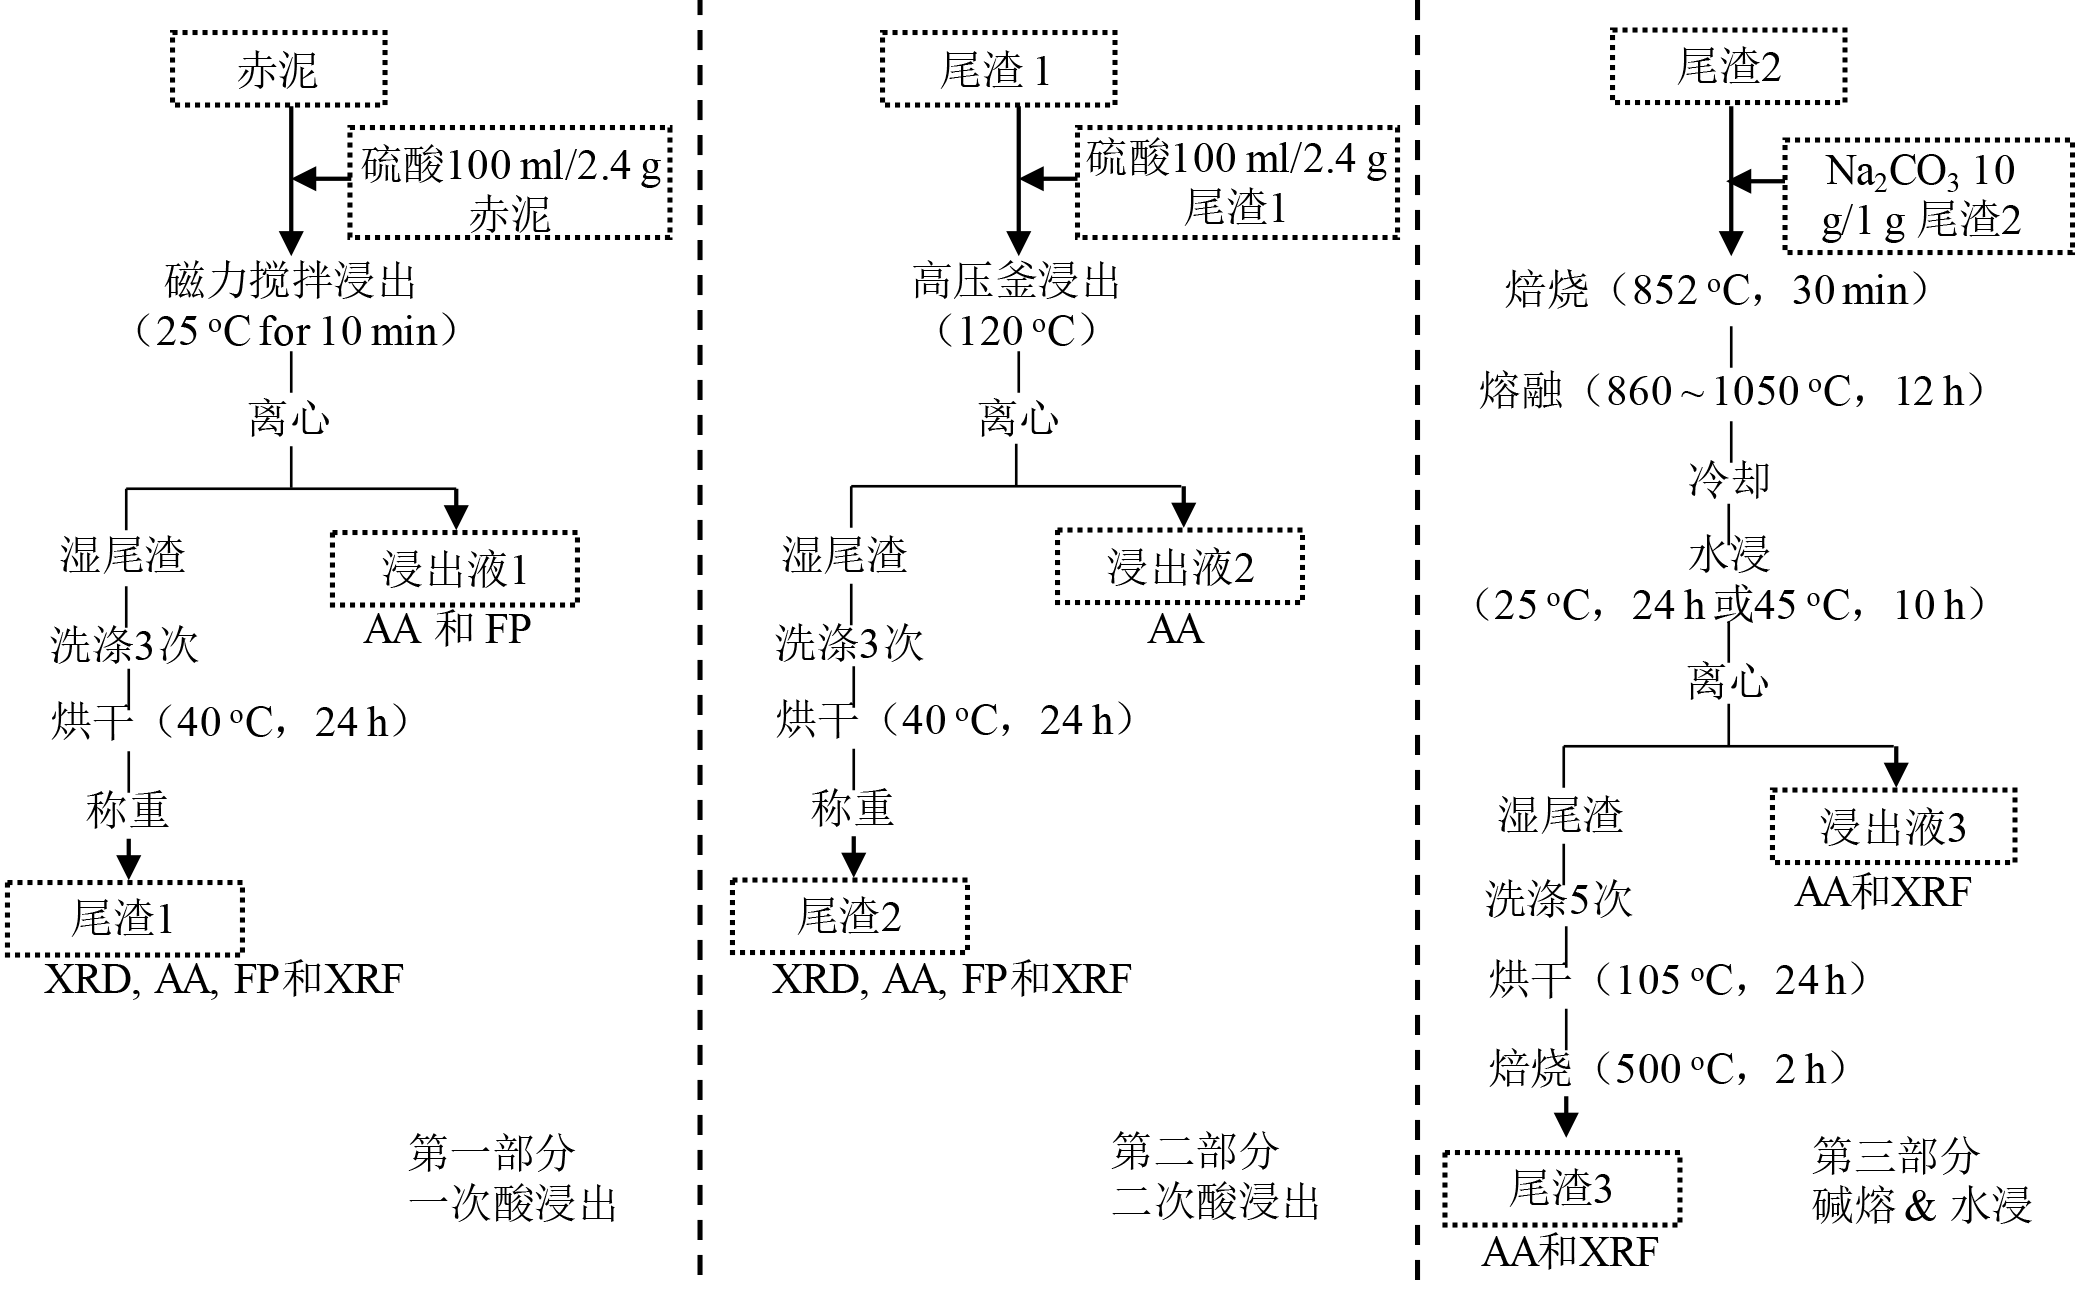
\includegraphics[width=\linewidth]{Figures/c1/Figure9}
	\caption{分步回收赤泥中钛锆流程图}\label{recoveringTiZr}
\end{figure}

Cyanex 301和Cyanex 302溶剂也就是二(2,4,4-三甲基戊基)二硫代次膦酸和二(2,4,4-三甲基戊基)单硫代次膦酸可用于一些普遍存在Mg$ ^{\mathrm{2+}} $、Mn$ ^{\mathrm{2+}} $、Fe$ ^{\mathrm{3+}} $、Al$ ^{\mathrm{3+}} $、Ce$ ^{\mathrm{4+}} $、V$ ^{\mathrm{5+}} $离子液中提钛\cite{deep2001extraction}。Ti$ ^{\mathrm{4+}} $离子在pH 1.0 \textasciitilde{ }1.6容易被萃取分离出来,再通过0.1 M草酸或3 \% H$ _{\mathrm{2}} $O$ _{\mathrm{2}} $-0.5 M H$ _{\mathrm{2}} $SO$ _{\mathrm{4}} $中选择性的分离上一步共同萃取出的Fe$ ^{\mathrm{3+}} $。反萃取有机相可通过用0.1 M草酸和0.1 M果酸分别除去Fe$ ^{\mathrm{3+}} $和Al$ ^{\mathrm{3+}} $,进一步净化。在这些萃取步骤中大量的有机酸会因此而消耗;另外,在用酸浸出赤泥中的各离子时也会耗用大量的酸。二(2-乙基己基)磷酸(D2EPHA, H$ _{\mathrm{2}} $A$ _{\mathrm{2}} $)是另外一个可以从硫酸介质\cite{islam1981solvent}或氯化物介质溶液\cite{islam1981solvent,biswas1998solvent}中有效提取4价钛的溶剂。在氯化物溶液中,下面的反应表示了钛的负载过程,负载效率不受氯化物浓度影响。
\begin{equation}
{\rm{Ti}}{{\rm{O}}^{{\rm{2 + }}}}{\rm{ + 2}}{{\rm{H}}_{\rm{2}}}{{\rm{A}}_{\rm{2}}} = {\left[ {{\rm{TiO}}{{\left( {{\rm{H}}{{\rm{A}}_{\rm{2}}}} \right)}_{\rm{2}}}} \right]_{{\rm{(O)}}}}{\rm{ + 2}}{{\rm{H}}^{\rm{ + }}}
\end{equation}

钒的原子序数为23,是一种重要的化学元素。由于其良好的延展性、硬度和疲劳强度,钒已被广泛商业应用于铁及非铁合金中,包括钢轨、工具钢、催化剂和航天航空材料\cite{moskalyk2003processing}。氧化钒可通过炭吸附与解析附路径进行回收\cite{mukherjee1990recovery}。在这个工艺中,赤泥首先在热水中混溶30 min后,然后用活性炭在pH  \textasciitilde{ }2.5,温度 \textasciitilde{ }80 \textcelsius 条件下进行吸附;然后在85 \textcelsius 含10 \%氨水中解析附饱和负载钒的活性炭,并生成含钒铵盐沉淀物;最后,含量高达99.9 \%的钒可以通过煅烧含钒铵盐得到。工艺流程示意图如图\ref{recoveringV2O5}所示。

到目前为止,这些关于回收钒钛的工艺流程都主要是在实验室内完成的。也就是说这些工艺都还没有大规模工业化应用或商业应用。此外,大规模的商业应用还需要赤泥或其他资源的供应源源不断。所以为了能够最大盈利,钒钛提取或分离工厂应该建立在氧化铝厂或赤泥渣场附近。否则,由于运输产生的交通费用而增加了提取成本,相比于从自然界其他矿物中钒钛的提取工艺其竞争性更差。
\begin{figure}[!h]
	%\setlength{\abovecaptionskip}{0pt}%设置标题前距离,图片一般不用设置。
	\centering
	%\setlength{\abovecaptionskip}{10pt plus0.3ex minus 0.06ex}
	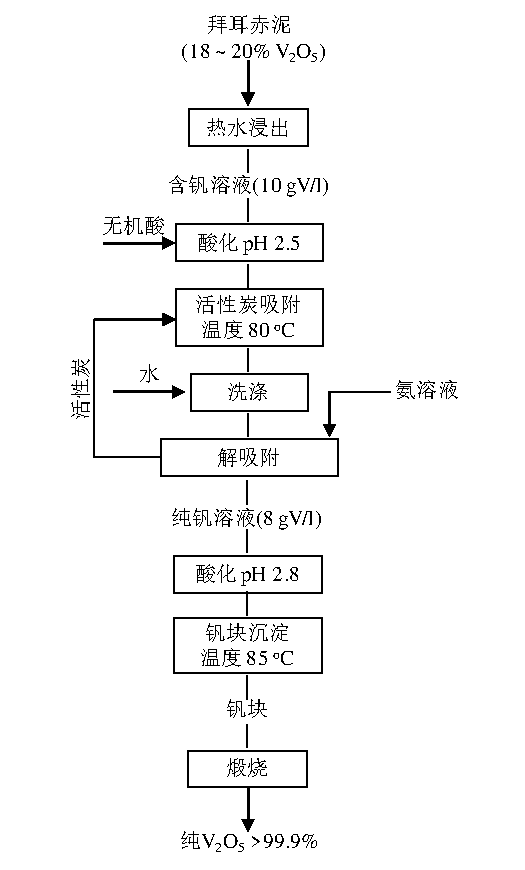
\includegraphics[width=0.65\linewidth]{Figures/c1/Figure10}%width=0.7大概为原来的100%。
	%\hspace{2pt}\includegraphics[width=0.45\linewidth]{Figures/Fig2}%\hspace设置水平间距
	\caption{炭吸附法回收赤泥中高纯钒氧化物}\label{recoveringV2O5}
\end{figure}

\begin{table}[!htbp]
	\centering
	%\setlength{\abovecaptionskip}{18pt plus 0.03ex minus 0.6ex}
	\setlength{\belowcaptionskip}{12pt plus 0.6ex minus 0.03ex}
	\xwu
	\begin{threeparttable}
		\caption[赤泥中部分微量元素化学组成及其赋存形态]{赤泥中部分微量元素化学组成及其赋存形态 (ppm)}\label{rareelements}
		\renewcommand\arraystretch{1.2}%设置行距距
		\begin{tabularx}{\linewidth}{p{1.9cm}p{1.4cm}p{1.3cm}XXXXXp{1.5cm}}%p{20pt}指定宽度。
			\toprule[1.5pt]
			元素&Sc&Y&Ga&V&Cr&U&Th&REEs\\\midrule
			澳大利亚&54&68&89&730&497&$\times$&$\times$&$\times$\\
			中国贵州&158&266&570&4220&848&59&201&2600\\
			希腊Pechiney&60.6&60.1&$\times$&$\times$&$\times$&$\times$&$\times$&$\times$\\
			希腊  &$\times$&$\times$&$\times$&1600$ \mathrm{^{a}} $ &2800$ \mathrm{^{a}} $ &$\times$&$\times$&$\times$\\
			印度&50&10&$\times$&6800&$\times$&$\times$&$\times$&$\times$\\
			印度Alcan&130\textasciitilde 162$ \mathrm{^{a}} $&$\times$&$\times$&$\times$&$\times$&$\times$&$\times$&$\times$\\
			前苏联&60\textasciitilde 250$ \mathrm{^{a}} $&$\times$&$\times$&$\times$&$\times$&$\times$&$\times$&$\times$\\
			通常范围&60\textasciitilde 120&60\textasciitilde 150&60\textasciitilde 80&$\times$&$\times$&50\textasciitilde 60&20\textasciitilde 30&355\textasciitilde 1400$ \mathrm{^{a}} $\\\midrule
			赋存形态&类质同象\\
			\bottomrule[1.5pt]
		\end{tabularx}\vspace{4pt}
		\footnotesize $ \times $:没找到;$ \mathrm{^{a}} $:以氧化物形式计算。
	\end{threeparttable}
\end{table}
\subsection{赤泥中钪镓的回收}
钪是一种高度分散的微量元素,一般赋存于火成岩中。它可以从铀和钨等其他金属提取后的尾矿或浸出液中以副产物形式提取分离出来\cite{roosen2016recovery}。
S. Xu和S. Li\cite{shaoquan1996review}指出当矿石中含钪品位达到20 ppm\footnote{parts per million}时,就具有商业开采价值。然而在大部分的铝土矿中,通常都含有微量的钪和镓等稀贵金属。在拜耳法处理铝土矿后,赤泥中钪的含量还会再次富集,其浓度甚至可为原来铝土矿的两倍\cite{ochsenkuhn1994direct}。有价元素镓却由于其物化性质与铝类似,大部分镓经过拜耳工艺后溶于母液中作为提铝副产物而被回收,所以一般不到30 \%的镓还残留在赤泥渣中\cite{liu2015metallurgical}。对于钪来说,赤泥是提取这类稀贵金属的重要潜在资源。在钪资源方面,不仅稀少,而且其市场价格较贵。例如,99.9 \% (3N)纯度的钪锭和99.99 \% (4N)纯度的Sc$ _{\mathrm{2}} $O$_{\mathrm{3}}$的市场价格分别是134 US\$$\cdot$g$ ^{\mathrm{-1}} $和5.1 US\$$\cdot$g$ ^{\mathrm{-1}} $\cite{ober2016mineral}。表\ref{priceofScandGa}总结出了近10年关于Sc$ _{\mathrm{2}} $O$_{\mathrm{3}}$和Ga的市场价格\cite{ober2016mineral,Brian2011mineral}。在2012年时,表中钪的价格从当初不到1900 \$$\cdot$kg$ ^{\mathrm{-1}} $迅猛增涨到4926 \$$\cdot$kg$ ^{\mathrm{-1}} $。金属镓的价格在2006 \textasciitilde{ }2010年间基本稳定在700 \$$\cdot$kg$ ^{\mathrm{-1}} $左右;然而自2011年,价格从742 \$$\cdot$kg$ ^{\mathrm{-1}} $逐渐降到2015年的297 \$$\cdot$kg$ ^{\mathrm{-1}} $,其原因可能是智能手机LEDs等其他平板屏幕市场的需求和政府政策导向发生了变化。经过近20年的科学研究,钪的多种商业应用价值也已经开发出来了。例如,将钪参杂到铝中,可使得到的铝钪合金强度更大,质量更轻,耐热与耐腐蚀性更好,这样的合金可应用于航空航天设备和高端体育器械。此外,钪在固态氧化物燃料电池(SOFCs\footnote{solid oxide fuel cells})方面,也表现出极好的导电性和热稳定性\cite{irvine2005scandia}。
\begin{table}[!htbp]
	\centering
	\wu
	\renewcommand\arraystretch{1.2}
	\begin{threeparttable}
		\vspace{-5pt}
		\caption[近十年氧化钪和金属镓的市场价格]{近十年氧化钪和金属镓的市场价格(\$$\cdot$kg$ ^{\mathrm{-1}} $)}\label{priceofScandGa}
		\begin{tabularx}{\linewidth}{p{1.7cm}XXXXXXXXXX}
			\toprule[1.5pt]
			时间&2006&2007&2008&2009&2010&2011&2012&2013&2014&2015\\\midrule
			Ga价格1&443&530&579&449&670&688&529&502&363&295\\
			Ga价格2&532&621&652&505&734&742&554&517&368&297\\
			Sc价格1&1450&1620&1620&1620&1620&1620&4700&5000&5400&5100\\
			Sc价格2&1743&1899&1824&1823&1774&1748&4926&5151&5481&5137\\
			\bottomrule[1.5pt]
		\end{tabularx}\vspace{4pt}
		{\footnotesize 注意:价格1为当年的市场价格;价格2为相对于2016年第三季度CPI居民消费价格指数值。Ga是指纯度为6 N的镓锭;Sc是指纯度为4 N的Sc$ _{\mathrm{2}} $O$ _{\mathrm{3}} $。}
	\end{threeparttable}
\end{table}

自然界铝土矿中或多或少的含有一定量的钪氧化物。拜耳工艺处理铝土矿后,存在于赤泥当中钪通常就变为了原矿的两倍\cite{ochsenkuhn1994direct}。大多数钪以类质同像的形式存在于赤泥中或铝土矿中\cite{xiao1996distribution,Chi1993scandium},品位在60 \textasciitilde{ }120 ppm之间,如表\ref{rareelements}所示\cite{smirnov1997investigation,samouhos2013greek,xiao1996distribution,ochsenkuhn2002pilot,wang2013recovery,sinha2014extraction}。部分其他不同国家的赤泥微量元素含量数据也列出在表\ref{rareelements}中。一般地认为,当矿物中的钪大于0.002 \% (20 ppm)时,那么该矿物就具有开采价值,是钪的重要资源\cite{shaoquan1996review}。牙买加的铝土矿中Sc$ _{\mathrm{2}} $O$ _{\mathrm{3}} $含量在87 \textasciitilde{ }113 ppm范围之间,然而在赤泥中Sc$ _{\mathrm{2}} $O$ _{\mathrm{3}} $含量就富集到了200 \textasciitilde{ }390 ppm \cite{wagh1987occurrence}。在希腊,干燥的赤泥中钪含量通常有130 ppm或约0.02 \% Sc$ _{\mathrm{2}} $O$ _{\mathrm{3}} $\cite{ochsenkuhn1994direct}。这些统计数据表明,赤泥中的钪含量往往都高于其开采价值的最低含量要求,也就是说赤泥是一种具有潜在钪资源开采价值的矿物。在赤泥中,钪含量除了较小之外,还含有大量的氧化铝,二氧化硅,铁、钛氧化物,所以从赤泥中直接回收钪并不是件容易的事。
\begin{figure}[!h]
	\centering
	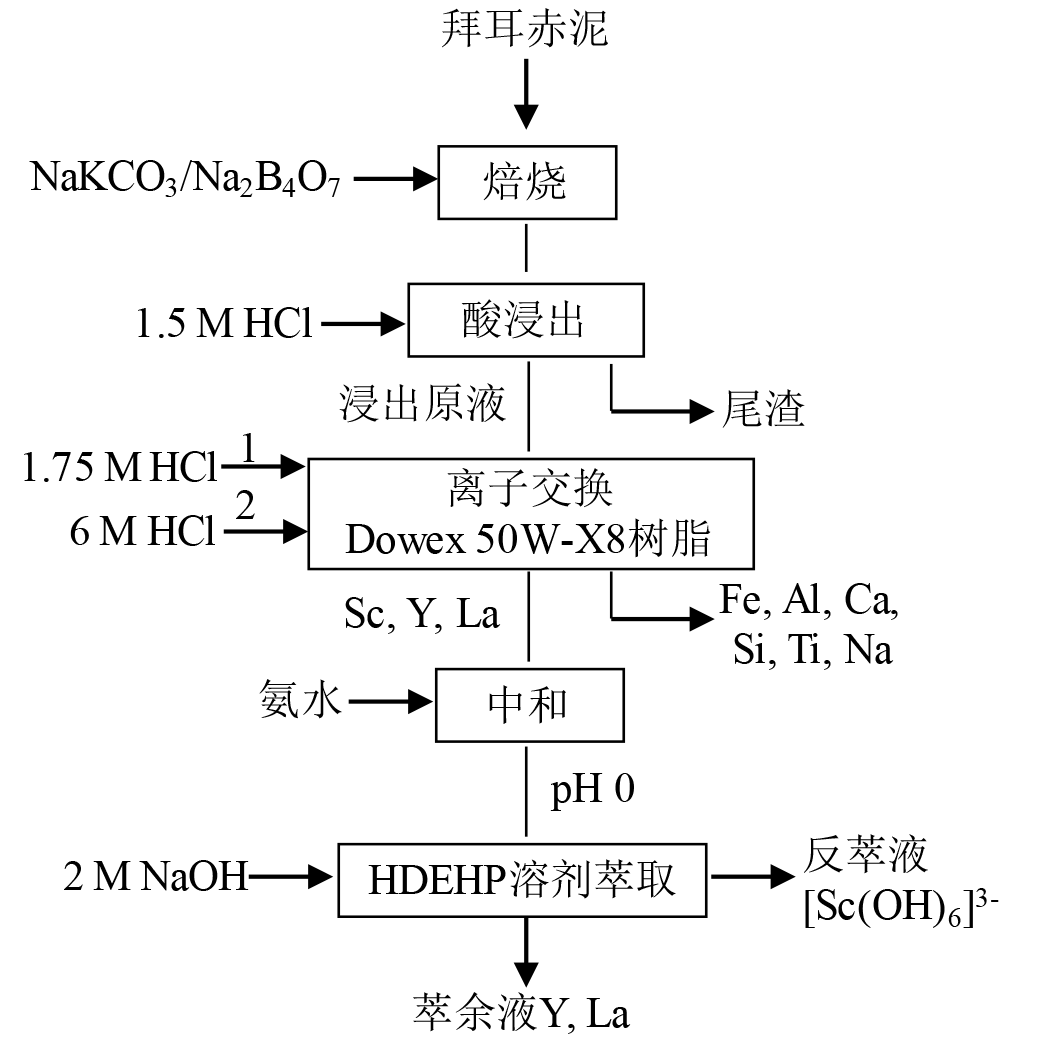
\includegraphics[width=0.65\linewidth]{Figures/c1/Figure11}%width=0.7大概为原来的100%。
	\caption{赤泥中回收钪的实验室研究流程图}\label{recoveringSc}
\end{figure}

0.25体积分数的活性炭在60 \textcelsius 磷酸三丁酯TBP—6 M HCl 溶液中处理改良4 h后,可用于钪的选择性吸附\cite{hualei2008extraction}。吸附完后,吸附剂和被吸附物通过洗涤过滤分离。实验结果还表明最优吸附条件是用 \textasciitilde{ }6.25 g$ \cdot $L$ ^{\mathrm{-1}} $吸附剂在35 \textcelsius 吸附40 min;另外,化学反应是活性炭吸附钪的主要控制步骤。吸附机制可用如下方程式表示\cite{hualei2008extraction}。
\begin{equation}
\left( {{\rm{2}} - {\rm{3}}} \right){\rm{PO}} + {\rm{S}}{{\rm{c}}^{{\rm{3 + }}}} + {\rm{3}}{\rm{C}}{{\rm{l}}^ - }{\rm{  =  }}\left( {{\rm{2}} - {\rm{3}}} \right){\rm{PO}} \cdot {\rm{ScC}}{{\rm{l}}_{\rm{3}}}
\end{equation}

此处的PO表示改良后活性炭的有效活性位置。从方程式中可以看到吸附过程中每个钪离子需要消耗两个有效活性位置。Hubicki\cite{hubicki1990studies}用选择性离子交换柱成功地把钪从稀土元素中分离了出来,然后再用6 M HCl把钪富集到500 g$ \cdot $L$ ^{\mathrm{-1}} $。除了传统的吸附剂之外,功能型多孔杂化材料对重稀土元素也表现出了良好的选择吸附性\cite{florek2014nanostructured}。
\begin{figure}[!h]
	%\setlength{\abovecaptionskip}{0pt}%设置标题前距离,图片一般不用设置。
	\centering
	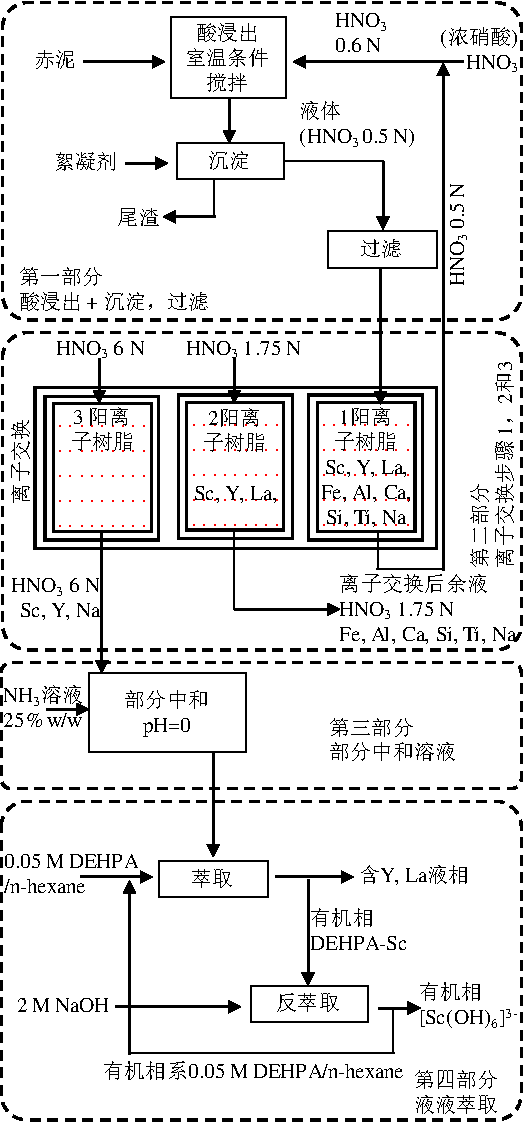
\includegraphics[width=0.65\linewidth]{Figures/c1/Figure12}%width=0.7大概为原来的100%。
	\caption{赤泥提钪中试流程图}\label{recoveringSc-middlescale}
\end{figure}

Ochsenkuhn-Petropulu\cite{ochsenkuhn1995selective}等人首先提出了离子交换 — 溶剂萃取的提钪方法,其工艺流程示意图如图\ref{recoveringSc}所示。赤泥和NaKCO$ _{\mathrm{3}} $/Na$ _{\mathrm{2}} $B$ _{\mathrm{4}} $O$ _{\mathrm{7}} $ (1:1)的混合料(赤泥:NaKCO$ _{\mathrm{3}} $:Na$ _{\mathrm{2}} $B$ _{\mathrm{4}} $O$ _{\mathrm{7}} $ = 2:1:1) 在1100 \textcelsius 下焙烧20 min,再用1.5 M HCl浸出。一半的浸出液在15 mL Dowex 50W-X8树脂柱中进行离子交换实验。离子交换树脂上的主要元素Fe、Al、Ti、Na、Si、Ca和微量元素Ni、Cr、Mn和V可用150 mL的1.75 M HCl洗脱掉。离子交换树脂上钪和其他杂质如钇和镧系元素可用6 M HCl 100 mL洗脱掉。随后再用0.05 M二(2-乙基己基)磷酸(DEHPA, (RO)$ _{\mathrm{2}} $POOH,  R是C$ _{\mathrm{8}} $H$ _{\mathrm{17}} $)无极性己烷溶剂选择性萃取出钪,在萃取之前需用NH$ _{\mathrm{4}} $OH将pH调到 \textasciitilde{ }0。萃取过程中,DEHPA主要以(HL)$ _{\mathrm{2}} $二聚分子存在,萃取机理如下所示\cite{ochsenkuhn1995selective,forsberg1983gmelin}。
\begin{equation}
{\rm{Sc}}_{{\rm{aq}}}^{{\rm{3 + }}}{\rm{ + 3}}{\left( {{\rm{HL}}} \right)_{{\rm{2org}}}} \leftrightharpoons {\rm{Sc}}{\left( {{\rm{LHL}}} \right)_{{\rm{3org}}}}{\rm{ + 3H}}_{{\rm{aq}}}^{\rm{ + }}
\end{equation}

为了保证阳离子交换反应可行,酸度应小于1 M,钪络合物与萃取剂比值应该小于10$ ^{\mathrm{-3}} $。萃取之后,用2 M NaOH溶液在5 min内可以Sc(OH)$ _{\mathrm{6}}^{\mathrm{3-}} $形态反萃取93 $ \pm $ 5 \%钪。

图\ref{recoveringSc-middlescale}是基于上述实验室结果的中式规模提钪示意图\cite{ochsenkuhn2002pilot}。赤泥首先直接用0.6 N的稀硝酸常温常压溶解,这个步骤具体一定的选择性,在液固比小于4 \%时,十分有利于钪的溶出而不利于铁的溶出。这里需要注意的一点是钪和铁离子由于其离子半径相近在溶液中较难分离\cite{ochsenkuhn1996recovery}。在浸出过程中,基于未反应核模型的钪浸出率$ \eta\mathrm{_{Sc}} $可表示为如下等式。
\begin{equation}
{\eta \rm{_{Sc}}} = \frac{{\rm{15.03}}}{{\left( {{{{\mathit{M_d}}} \mathord{\left/
					{\vphantom {{{\mathit{M_d}}} \mathit{V}}} \right.
					\kern-\nulldelimiterspace} \mathit{V}}} \right){\mathit{C}_{\rm{{Sc,RM}}}}}}\left[ {{\rm{1}} - {{\rm{0.00635}}^{\left( {{{{\mathit{M_d}}} \mathord{\left/
						{\vphantom {{{\mathit{M_d}}} \mathit{V}}} \right.
						\kern-\nulldelimiterspace} \mathit{V}}} \right)\textit{w}}}} \right]
\end{equation}

\textit{M$ _\mathit{d} $}/\textit{V}表示干燥赤泥量与浸出液比值,kg$\cdot$L$^{\mathrm{-1}}$;\textit{C}$ \rm{_{Sc,RM}} $表示赤泥中钪的质量分数(w/w),mg$\cdot$kg$^{\mathrm{-1}}$;\textit{w}尺寸矫正一元运算符, L$\cdot$kg$ ^{\mathrm{-1}} $。通过研究搅拌模式、固液比 、浸液酸度和浸出时段对钪浸出影响,发现当\textit{M$ _d $}/\textit{V}小于0.1,pH值为0 \textasciitilde{ }0.2,第一浸出阶段搅拌充足时可以获得最大的\textit{C}$ _{\mathrm{Sc}} $/\textit{C}$ _{\mathrm{Fe}} $比值。虽然,离子交换法提钪可行,但它并不是最明智的做法。因为大量的其他金属元素杂质如Fe、Ti和Al会极大影响树脂效率\cite{wang2011separation}。在后面的章节中会有更深入的解释。

W. Wang\cite{wang2013recovery}等人提出了一种从澳大利亚赤泥中酸浸—溶剂选择性萃取钪的方法。浸出结果表明在相同的浸出条件下(固液比0.05,浸出温度23 \textcelsius,浸出时间120 min),0.5 M稀硫酸与相同浓度的HNO$ _{\mathrm{3}} $或HCl相比,钪浸出性较好。0.05 M二乙基己基磷酸(D2EHPA)-0.05 M 磷酸三丁酯TBP萃取系在众萃取系中萃取性能最好。在萃取钪前,用0.025 M伯胺(Primene JM 1,1,3,3,5,5,7,7,9,9-十甲基癸胺)—壳牌D70的溶剂油在A/O比为5,pH 0.2 \textasciitilde{ }0.5,40 \textcelsius 条件下可先分离大于99 \% Zr和40 \%的Ti\cite{wang2013recovery}。图\ref{recoveringScbywangweiwei}是从赤泥中基于上述方法回收钪的工艺路线图。
\begin{figure}[!h]
	%\setlength{\abovecaptionskip}{0pt}%设置标题前距离,图片一般不用设置。
	\centering
	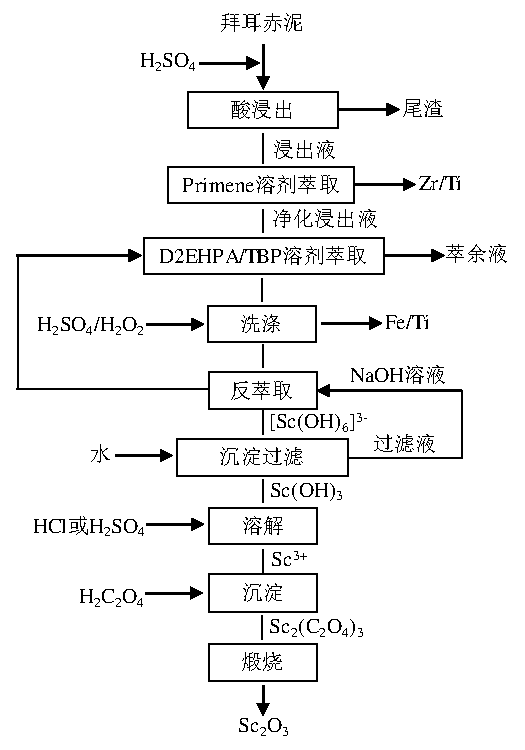
\includegraphics[width=0.65\linewidth]{Figures/c1/Figure13}%width=0.7大概为原来的100%。
	%\hspace{2pt}\includegraphics[width=0.45\linewidth]{Figures/Fig2}%\hspace设置水平间距
	\caption{赤泥中回收钪的理想流程图}\label{recoveringScbywangweiwei}
\end{figure}

将二氧化碳充入赤泥浆中可促进钪的浸出\cite{yatsenko2010red}。向赤泥浆中充入二氧化碳,一方面可以让赤泥中强碱相转变为碳酸盐或碳酸氢盐,减小由于堆置对周围环境产生的影响;另一方面可以减小二氧化碳引起的温室效应。除此之外,若将赤泥经过旋风分离器一次分离富集钪后,再经过浸出、萃取、反萃取和沉淀后,可使钪的回收率达到75 \%以上\cite{xiu_fen2003summarization}。在浸出步骤中,除了硝酸之外,还可用碳酸钠,50 \%的硫酸以及3 M的盐酸溶液浸出赤泥中的钪。

镓是一种地球岩石圈中广泛分布丰度为10 g$ \cdot $t$ ^{\mathrm{-1}} $的稀有金属元素\cite{poledniok2008speciation}。由于镓与铝的亲和性,所以在铝土矿中通常与铝伴生存在。在目前现有技术中,从任何一种矿物中直接提取镓,其成本都是高于镓本身价值的。因此,镓通常是氧化铝或锌生产过程中的副产品。在拜耳法工艺中,铝土矿浸出液中的镓含量约占铝土矿镓总量的70 \%,仅有 \textasciitilde{ }30 \%的镓未溶解残存于赤泥中。据有效数据统计,世界上大概90 \%的镓都产自于拜耳液\cite{lu2008research}。从拜耳液中回收镓的主要方法有分段沉淀、点化学沉积、溶剂萃取和离子交换法。其中,溶剂萃取和离子交换法相比于其他方法有较好的提取性能\cite{zhao2012recovery}。但是,从赤泥中提取镓的研究报道却基本上没有。

由于赤泥中钪和镓的含量极低,从赤泥中直接酸浸提取钪或镓很显然是不可行的。因为在浸出过程中,大多数杂质元素Fe、Ca、Al、Ti、Na、Si等大量溶于酸中,随后在柱浸实验中被共同吸附于树脂上,不仅影响钪和镓从浸出液中分离,而且降低了树脂负载效率。另外,在树脂吸附过程后,一般还需大量的酸清洗树脂上杂质,中和废酸清洗液又需要消耗大量的碱液,所以运行成本也会因此而增加。
\subsection{赤泥中其他金属的回收}
赤泥中除了含有微量的钪和镓,还有一些其他稀贵金属或放射性元素,例如钇(60 \textasciitilde{ }150 g$ \cdot $t$ ^{\mathrm{-1}} $)、铀(50 \textasciitilde{ }60 g$ \cdot $t$ ^{\mathrm{-1}} $)、钍(20 \textasciitilde{ }30 g$ \cdot $t$ ^{\mathrm{-1}} $)等\cite{smirnov1997investigation,borra2015leaching},相关数据都列出在表\ref{rareelements}中。在风轮机、混合动力汽车、国防应用等一些产品中掺杂一定量的稀土元素后可以极大的提高终产品的性能,有些性能甚至是其他材料不可替代的。在近15年中,由于各行业的发展,稀土矿物储存减少以及社会对稀土元素的需求快速增长,从赤泥中回收稀土元素也引起了越来越大的关注\cite{du2011global}。

赤泥中钪和铀可通过硫酸浸出树脂吸附法回收\cite{smirnov1997investigation}。含氮磷两性树脂AFI-21和AFI-22是可用于钪和铀的离子吸附。在吸附过程中,pH值大小对离子交换器的吸附能力有明显影响,实验中选定的pH值研究范围是0.9 \textasciitilde{ }1.5,以降低对铝的吸附能力和酸的消耗。钪离子在pH为0.5 \textasciitilde{ }4.0主要以水解阳离子Sc(H$ _{\mathrm{2}} $O)$ _{\mathrm{6}}^{\mathrm{3+}} $的形式存在,增大pH值将使其转变为伪胶体形态。实验结果发现:除了50 \%钪可从硫酸浆赤泥中浸出回收外,部分放射性元素铀和钍也被吸附出来,得到的含5 \textasciitilde{ }7 \% Sc,4.5 \% U,0.9 \% Th的滤渣。另外,钛也会在开始的浸出液中水解出来,富集在沉淀滤饼中,其中钛含量在35 \textasciitilde{ }40 \%之间。Fulford(Patent US5015447 A)等人将SO$ _{\mathrm{2}} $充入赤泥中进行选择性地浸出了原子序数为57 \textasciitilde{ }71稀土元素、钪和钇。在此方法中,铁钛几乎没有溶出。赤泥用稀亚硫酸溶液在1.8 \textasciitilde{ }3.2间消解,可以得到含稀土元素和少量杂质的浸出液。若分两段消解,在pH为2.6 \textasciitilde{ }3.2时,方钠石类矿物中钠、铝、硅将溶进浸出液;在pH降低到1.8 \textasciitilde{ }2.5时,稀土元素和部分方钠石类矿物元素浸出。此阶段若再细分为pH 2.0 \textasciitilde{ }2.4 和1.5 \textasciitilde{ }2.0两个阶段时,目标浸出液中含有的杂质元素就更少了。在浆液pH为2.0时,不分阶段一次性浸出,则苏打、氧化铝和二氧化硅等杂质也会随着稀土元素的浸出而浸出。浸出液中目标元素再经过溶剂萃取和不同pH值反萃取而回收。溶液中钪的提取可通过DEHPA,2-乙基己基磷酸单2-乙基己基脂(EHEHPA),二(2,4,4-三甲基戊基)次膦酸(Cyanex 272),二(2,4,4-三甲基戊基)二硫代次膦酸(Cyanex 301)及其混合剂,与磷酸三丁酯(TBP)或三正辛基氧膦(TOPO)或煤油的有机稀释剂组成的萃取系萃取分离实现。通常,三正辛基氧膦TOPO将会降低溶剂对轻稀土、重稀土和中稀土(除了钇)的萃取能力。具体相关溶剂萃取与特性能总结在表\ref{selectivity of solvent}中\cite{wang2011separation,Recovery1989}。在目前描述的研究结果中,尽管稀土元素可从赤泥中浸出,但从铝土矿中用稀矿物酸却一般不行。SO$ _{\mathrm{2}} $提钪法的另外一个优点就是在浸出过程中大部分的SO$ _{\mathrm{2}} $或SO$ _{\mathrm{3}} $可以回收再利用。若在25 \textcelsius,24 h,固液比1:50的浸出条件下,用0.5 M的稀硝酸可浸出赤泥中 \textasciitilde{ }60 \%重稀土(Dy, Er, Yb),\textasciitilde{ }50 \%中稀土(Nd、Sm、Eu、Gd),\textasciitilde{ }30 \%轻稀土(La、Ce、Pr),96 \%钇和80 \%的钪\cite{ochsenkuhn1996recovery}。但与此同时,浸出体系对赤泥中主要成分特别是对铁的溶解能力却表现平平, 仅\textasciitilde{ }3 \%的Fe发生溶解。在没有杂质铁的干扰下,用电感耦合等离子体原子发射光谱法测量镧系和钇时的准确度也提高了。若用0.5 M的HCl浸出赤泥时,钪和钇的浸出率较0.5 M的HNO$ _{\mathrm{3}} $小。

\begin{sidewaystable}[!htbp]
	\centering
	\vspace{10pt}
	\setlength{\belowcaptionskip}{-12pt plus 0.6ex minus 0.03ex}
	\xwu
	\begin{threeparttable}
		\caption{赤泥有价元素萃取常用溶剂}\label{selectivity of solvent}
		\renewcommand\arraystretch{1.05}%设置行距距
		\begin{tabularx}{\linewidth}{>{\hsize=0.25\hsize}X>{\hsize=0.6\hsize}X>{\hsize=0.7\hsize}XX}%p{20pt}指定宽度。
			\toprule[1.5pt]
			作用&酸浓度&萃取系及方法&萃取元素/选择性\\\midrule
			萃取&pH 1.5 \textasciitilde{ }2.0&0.05 \textasciitilde{ }0.1 M有机磷萃取剂&原子序数: 65 \textasciitilde{ }71, Y, 部分Gd, Nd, Ca\\
			萃取&pH 2.0 \textasciitilde{ }2.5&0.1 \textasciitilde{ }0.2 M 有机磷萃取剂&原子序数: 57 \textasciitilde{ }63, 部分Ca, Al\\
			萃取&pH 1.5 \textasciitilde{ }2.0 &0.2 \textasciitilde{ }0.3 M 有机磷萃取剂&原子序数: 57 \textasciitilde{ }71, Sc, Y, 部分Ca, Al\\
			萃取&1 \textasciitilde{ }11 M HCl, HClO$_{\mathrm{4}}$ 或 HNO$_{\mathrm{3}}$&0.75 M HDEHP-正庚烷或环己烷&Sc$^{\mathrm{3+}}$ \textasciitilde{ }Ti$^{\mathrm{4+}}$, Zr$^{\mathrm{4+}}$, Hf$^{\mathrm{4+}}$$>$ Y$^{\mathrm{3+}}$$>$La$^{\mathrm{3+}}$$>$Mn$^{\mathrm{2+}}$\\
			萃取&3 \textasciitilde{ }10 M HCl&HDEHP-正辛烷&Sc$^{\mathrm{3+}}$$ \gg $Fe$^{\mathrm{3+}}$$>$Lu$^{\mathrm{3+}}$$>$Yb$^{\mathrm{3+}}$ $>$Er$^{\mathrm{3+}}$$>$Y$^{\mathrm{3+}}$$>$Ho$^{\mathrm{3+}}$\\
			萃取&0.5 M HCl &20 \% HDEHP, 15 \% TBP-煤油&Sc$^{\mathrm{3+}}$$>$Fe$^{\mathrm{3+}}$$>$Al$^{\mathrm{3+}}$$>$Mg$^{\mathrm{2+}}$\\
			萃取&pH 1.5 \textasciitilde{ }3.5 H$_{\mathrm{2}}$SO$_{\mathrm{4}}$&0.2 M D2EHPA and 1 \% TBP-Escaid 110&Sc$^{\mathrm{3+}}$ \textasciitilde{ }Zn$^{\mathrm{2+}}$$>$Ca$^{\mathrm{2+}}$ \textasciitilde{ }Al$^{\mathrm{3+}}$$>$Mn$^{\mathrm{2+}}$$>$Cr$^{\mathrm{3+}}$ \textasciitilde{ }Mg$^{\mathrm{2+}}$ \textasciitilde{ }Ni$^{\mathrm{2+}}$ \textasciitilde{ }Si\\
			萃取&0.5 \textasciitilde{ }11 M HClO$_{\mathrm{4}}$&0.1 M HDEHP-甲苯&Sc$^{\mathrm{3+}}$$>$Fe$^{\mathrm{3+}}$$>$Al$^{\mathrm{3+}}$$>$Mg$^{\mathrm{2+}}$\\
			萃取&0.5 \textasciitilde{ }1.5 M H$_{\mathrm{2}}$SO$_{\mathrm{4}}$&Purified HEHEHP-正庚烷&Sc$^{\mathrm{3+}}$ \textasciitilde{ }Th$^{\mathrm{4+}}$$>$Ce$^{\mathrm{4+}}$$>$Fe$^{\mathrm{3+}}$\\
			萃取&1.5 \textasciitilde{ }5 M H$_{\mathrm{2}}$SO$_{\mathrm{4}}$&Purified HEHEHP-正庚烷&Sc$^{\mathrm{3+}}$$>$Ce$^{\mathrm{4+}}$$>$Th$^{\mathrm{4+}}$$>$Fe$^{\mathrm{3+}}$\\
			萃取&pH 1 \textasciitilde{ }5.5 H$_{\mathrm{2}}$SO$_{\mathrm{4}}$&HEHEHP 0.2 M Ionquest 801-1 \% TBP &Sc$^{\mathrm{3+}}$$>$Zn$^{\mathrm{2+}}$$>$Al$^{\mathrm{3+}}$$>$Mn$^{\mathrm{2+}}$ \textasciitilde{ }Cr$^{\mathrm{3+}}$ \textasciitilde{ }Ca$^{\mathrm{2+}}$ \textasciitilde{ }Mg$^{\mathrm{2+}}$ \textasciitilde{ }Ni$^{\mathrm{2+}}$ \textasciitilde{ }Si\\
			萃取&0.01 \textasciitilde{ }1 M HClO$_{\mathrm{4}}$&0.1 M HEHEHP-甲苯&Sc$^{\mathrm{3+}}$$>$Fe$^{\mathrm{3+}}$$>$Al$^{\mathrm{3+}}$$>$Mg$^{\mathrm{2+}}$\\
			萃取&3 \textasciitilde{ }10 M H$_{\mathrm{2}}$SO$_{\mathrm{4}}$&0.048 M Cyanex 272-己烷&Sc$^{\mathrm{3+}}$ \textasciitilde{ }Th$^{\mathrm{4+}}$$>$Fe$^{\mathrm{3+}}$$>$Lu$^{\mathrm{3+}}$\\
			萃取&pH  \textasciitilde{ }1 H$_{\mathrm{2}}$SO$_{\mathrm{4}}$ &0.1 M Cyanex 272-5 \% TBP&Sc$^{\mathrm{3+}}$$\gg$Al$^{\mathrm{3+}}$$>$Ni$^{\mathrm{2+}}$ \textasciitilde{ }Si$>$Mn$^{\mathrm{2+}}$ \textasciitilde{ }Mg$^{\mathrm{2+}}$ \textasciitilde{ }Ca$^{\mathrm{2+}}$$>$Cr$^{\mathrm{3+}}$\\
			萃取&3 \textasciitilde{ }10 M H$_{\mathrm{2}}$SO$_{\mathrm{4}}$&0.048 M Cyanex 302-己烷&Zr$^{\mathrm{4+}}$$>$Sc$^{\mathrm{3+}}$$>$Th$^{\mathrm{4+}}$$>$Fe$^{\mathrm{3+}}$$>$Lu$^{\mathrm{3+}}$\\
			萃取&3 \textasciitilde{ }10 M H$_{\mathrm{2}}$SO$_{\mathrm{4}}$&0.048 M Cyanex 301-己烷&Zr$^{\mathrm{4+}}$$>$Sc$^{\mathrm{3+}}$ \textasciitilde{ }Fe$^{\mathrm{3+}}$$>$Th$^{\mathrm{4+}}$$>$Lu$^{\mathrm{3+}}$\\
			萃取&7 \textasciitilde{ }8 M HCl&100 \% TBP&Sc$^{\mathrm{3+}}$ \textasciitilde{ }Zr$^{\mathrm{4+}}$$>$Th$^{\mathrm{4+}}$\\
			萃取&4 \textasciitilde{ }6 M HClO$_{\mathrm{4}}$&100 \% TBP&Sc$^{\mathrm{3+}}$$>$Zr$^{\mathrm{4+}}$\\
			萃取&5.8 M HCl&40 \% P350-煤油&Sc$^{\mathrm{3+}}$$>$Ti$^{\mathrm{4+}}$ \textasciitilde{ }Y$^{\mathrm{3+}}$ \textasciitilde{ }Al$^{\mathrm{3+}}$ \textasciitilde{ }Ca$^{\mathrm{2+}}$ \textasciitilde{ }Mg$^{\mathrm{2+}}$\\
			萃取&2.0 \textasciitilde{ }7.0 M H$_{\mathrm{2}}$SO$_{\mathrm{4}}$&5 \% Cyanex 923-煤油&Zr$^{\mathrm{4+}}$$>$Sc$^{\mathrm{3+}}$$>$Ti$^{\mathrm{4+}}$ \textasciitilde{ }Lu$^{\mathrm{3+}}$$>$Fe$^{\mathrm{3+}}$\\
			萃取&1 \textasciitilde{ }5 M HCl&5 \% Cyanex 923-煤油&Sc$^{\mathrm{3+}}$$>$Th$^{\mathrm{4+}}$$>$Lu$^{\mathrm{3+}}$\\
			萃取&2.0 \textasciitilde{ }7.0 M H$_{\mathrm{2}}$SO$_{\mathrm{4}}$&5 \% Cyanex 925-煤油&Zr$^{\mathrm{4+}}$$>$Sc$^{\mathrm{3+}}$$>$Lu$^{\mathrm{3+}}$$>$Ti$^{\mathrm{4+}}$$>$Fe$^{\mathrm{3+}}$\\
			萃取&0.5 \textasciitilde{ }2.5 M HCl&5 \% Cyanex 925-煤油&Th$^{\mathrm{4+}}$$>$Sc$^{\mathrm{3+}}$$>$ Lu$^{\mathrm{3+}}$\\
			萃取&1 \textasciitilde{ }5 M HCl&5 \% Cyanex 925-煤油&Sc$^{\mathrm{3+}}$$>$Th$^{\mathrm{4+}}$$>$Lu$^{\mathrm{3+}}$\\
			萃取& --&DEHPA/EHEHPA/Cyanex 272&轻稀土/重稀土\\
			提纯&0.1 \textasciitilde{ }0.2 M H$_{\mathrm{2}}$SO$_{\mathrm{3}}$或矿物酸&  --&Ca, La和最轻稀土\\
			提纯&1 \textasciitilde{ }3 M HNO$_{\mathrm{3}}$& --&原子序数: 51 \textasciitilde{ }71\\
			提纯&1 \textasciitilde{ }6 M HCl或H$_{\mathrm{2}}$SO$_{\mathrm{4}}$& --&原子序数: 51 \textasciitilde{ }71\\
			SO$_{\mathrm{2}}$回收&pH 2.4 \textasciitilde{ }3.0&H$_{\mathrm{2}}$SO$_{\mathrm{3}}$/加热&SiO$_{\mathrm{2}}$\\
			SO$_{\mathrm{2}}$回收&pH 3.2 \textasciitilde{ }4.0&H$_{\mathrm{2}}$SO$_{\mathrm{3}}$/加热&Al$_{\mathrm{2}}$O$_{\mathrm{3}}$\\
			\bottomrule[1.5pt]
		\end{tabularx}\vspace{0pt}
	\end{threeparttable}
\end{sidewaystable}

印度学者Abhilash通过硫酸浸出和溶剂萃取法从赤泥中提取了镧和铯\cite{sinha2014extraction}。用3 M H$ _{\mathrm{2}} $SO$ _{\mathrm{4}} $在固液比10 g$\cdot$L$ ^{\mathrm{-1}} $,搅拌时速200 rpm,35 \textcelsius 浸出条件下反应1 h,浸出液经过DEHPA或Cyanex 272或Cyanex 301萃取,高达99.9 \%的La可被回收;当浸出温度增加到75 \textcelsius 时,La的回收率却降到37 \%,但在用Cyanex 301萃取Ce时,回收率却高达99.9 \%。萃取过程中无论使用哪种溶剂都可将钪共同提取出来。

在生物浸出赤泥中稀土和放射性元素方面,真菌\textit{Penicillium tricolor}据报道可以实现这些元素的浸出\cite{qu2013bioleaching}。真菌新陈代谢的产物草酸和柠檬酸对生物浸出过程中螯合作用和络合作用起着重要作用。通过两步法——首先在蔗糖培养基中培养真菌72 h;产生大量真菌后再加入到消毒后的矿浆浓度为10 \% (w/v)赤泥浆中——20 \textasciitilde{ }75 \%的上述稀土或放射性元素可被浸出。在生物浸出赤泥中As、Ba、Cr、Cu、Ni、Pb元素方面,真菌\textit{aspergillus niger}对重金属显示出了的较好的溶解浸出能力,在矿浆浓度1 \% (w/v)时大多数元素可获得其最高浸出率\cite{qu2013bioleaching2}。

在酸浸提取赤泥有价元素过程中,一般需要使用大量的矿物酸如H$ _{\mathrm{2}} $SO$ _{\mathrm{4}} $、HNO$ _{\mathrm{3}} $、HCl或有机酸草酸、果酸等,浸出后大量的酸液若不能循环使用则需要中和处理。此外,对元素不具选择性或低选择性是这类直接酸浸方法的共性。


\section{课题的提出}
表\ref{conclusions}中总结了赤泥中主要有价元素的最佳回收率及其对应的相关工艺\cite{liu2009application,zhong2009extraction,vachon1994chemical,liu2012experimental,li2009recovery,uzun2007dissolution,eisele2014review,erccaug1997furnace,deep2001extraction,mukherjee1990recovery,ochsenkuhn2002pilot,sinha2014extraction,ochsenkuhn1995selective,ochsenkuhn1996recovery}。赤泥中有价元素的回收方法可大分为三类,也就是湿法冶金、火法冶金和生物冶金。目前研究中大部分方法可归为火法—湿法联合冶金。这些方法它们的共同点是对目标元素没有较强的选择性,同时导致了浸出液中金属离子浓度一般不能达到现行要求的零排放标准。生物湿法冶金与矿物酸浸处理赤泥相比,它的优势是更环保、灵活、低能耗,但生物培养周期往往较长、效率低;另外,pH和温度范围较窄导致其操作难度高。提取赤泥中有价元素时,不仅要考虑目标元素的提取效率,还应考虑焙烧或熔融、矿物酸浸、有机溶剂萃取、反萃取等各个环节的成本及其实际可行性。除此之外,工艺设计选用设备时,还应考虑其耐酸、耐碱、耐压性。

基本上所有的方法都采用无机酸或矿物酸作为有价元素特别是稀土元素的直接浸出剂,其最主要的缺点是对元素浸出不具有选择性,杂质金属元素和非金属元素硅的大量浸出。此外,化学浸出、萃取、反萃取过程中还会产生的大量废酸碱液和引起各种环境问题。当然这些工厂或企业最应该对这些药剂的使用而引起的或潜在的环境问题负责。湿法工艺处理赤泥产生的二次污染物、大量的酸耗、环境问题是其被限制运用的主要原因。在采用离子交换法单一提取赤泥中钪的方面,由于其较低的交换反应率,离子交换法提钪显得并不是十分可行;另外,由于杂质的影响,多次使用离子交换器后其效率也将受很大的影响。采用高温火法冶金如高温熔融或焙烧赤泥等原料则需消耗大量的能量。在回收铁的过程中,熔融或焙烧温度对生铁质量或渣中含铁量的多少影响较大。另外,温度对耐火材料的稳定性与渣铁分离度也相关。总之,赤泥应该被认为是一种重要矿物资源或建材原料,未来赤泥有机元素回收途径应该是环境友好、成本低廉和效率高效的。

由于赤泥中含有一定量的碱金属和碱土金属,不宜将没有处理过的赤泥仅因为铁品位较高而作为炼铁原料直接加入高炉中。这是因为碱金属和碱土金属将会富集循环于高炉内而腐蚀炉衬,同时还会增加高炉焦比。若仅考虑从赤泥中提取回收一种有价元素,这显然是不经济的。在实际当中,应该设计能够同时将Fe、Al、Na、Sc等多种有价元素分步提取或分离的工艺;然后再考虑把赤泥尾渣制备为或作为炼铁原料或建材原料或催化剂基体料或吸附剂等,以实现赤泥的完全资源化,减小了赤泥对环境的影响。

矿物成分和矿相组成对无机酸的选取及有价元素的回收都有重要影响,弄清赤泥中矿物成分和矿相组成十分有益于研究开发赤泥有价元素提取新途径。在未来的工作中,赤泥中微痕量元素赋存形态及特性应该被首先弄清和研究。微波加热、急冷,外场处理等赤泥预处理新方法也值得关注探究。另外,对于离子液体提取赤泥微量元素或其他有价元素工艺也是十分值得探究的。回收赤泥中有价元素对处理赤泥堆置引起的环境问题、铁矿石价格浮动、稀土资源的日益减少等问题都是十分重要和有意义的。一个生态环境友好型和高附加值赤泥综合利用工艺许多基础研究工作仍然值得相关研究人员们继续深入完善与探索。

如前所述,拜耳赤泥是最有期望价值的钪资源原料。如前所述,拜耳法赤泥是最有期望值的提钪资源,但对于传统火法—湿法冶金方法,若仅用于提取微量元素钪,由于其大量的能量消耗和复杂的赤泥中杂质元素预分离步骤(如离子交换)等因素而不合适,所以提钪的同时应考虑其他主要有价元素的综合回收。目前,火法—湿法冶金提取Al、Na、Ti、Sc和稀土元素工艺,通常包含研磨、焙烧、酸浸、溶剂萃取、沉淀及煅烧几个步骤。但是在分离目标元素的时候,其他共同浸出的元素将干扰后续的萃取反萃取过程。因此,在选用溶剂、方法、改良研发新的浸出系或萃取系时,应注意其在浸出和萃取时对目标元素的选择性。


\vspace{20pt}
\begin{center}
	%\renewcommand\arraystretch{1}%设置各大项(如Al和Na)之间的行间距
	%\setlength{\abovecaptionskip}{40pt}
	\setlength{\belowcaptionskip}{15pt plus 0.6ex minus 0.03ex}
	\tablecaption{赤泥中有价元素的最佳分离提取工艺\label{conclusions}}
	\tablefirsthead{%
		\toprule[1.5pt]\multicolumn{1}{l}{}&
		\multicolumn{1}{l}{回收工艺}&
		\multicolumn{1}{l}{最优结果}&
		\multicolumn{1}{l}{具体方法参数}&
		\multicolumn{1}{l}{工艺缺点}&
		\multicolumn{1}{l}{研究现状}\\\midrule}
	\tablehead{
		\multicolumn{6}{r}{续表\ref{conclusions}}\\\toprule[1.5pt]
		\multicolumn{1}{l}{}&
		\multicolumn{1}{l}{回收工艺}&
		\multicolumn{1}{l}{最优结果}&
		\multicolumn{1}{l}{具体方法参数}&
		\multicolumn{1}{l}{工艺缺点}&
		\multicolumn{1}{l}{研究现状}\\\midrule}
	\tabletail{\bottomrule[1.5pt]
		\multicolumn{6}{r}{接下页}\\}
	\tablelasttail{\bottomrule[1.5pt]}
\begin{spacing}{1}\wu%设置每项内的行间距和表里面的字体大小。
		\begin{supertabular}[!h]{p{0.3cm}p{1.6cm}p{1.5cm}p{4.1cm}p{2.4cm}p{1.2cm}}
			Al&湿法(水热碱浸法)&87.8\,\% Al&Al$_{\mathrm{2}}$O$_{\mathrm{3}}$ 浸出条件: 45\,\% NaOH溶液, CaO/赤泥 = 0.25, L/S = 0.9, 0.8 MPa, 200 \textcelsius, 3.5 h&操作难度高&实验室\\ 
			&&96.4\,\%\,Na&Na$_{\mathrm{2}}$O浸出条件:7\,\% NaOH 溶液, L/S = 3.8, 0.9 MPa, 170 \textcelsius, 2 h&&\\
			&生物浸出&75 \%&细菌\textit{P. Simplicissimum}酸性分泌液(酸浸), 3 h&效率低, 操作难度较高&实验室\\ 
			&火法—湿法&89.71 \%&还原性烧结: 1050 \textcelsius, 20 \textit{wt}\% 碳粉, 1.5 h; 浸出&能耗高&实验室\\
			Na&湿法(水热碱浸法)&90\,\%\,Na; 70\,\%\,Al&水热处理: 与CaO混匀后进行蒸气熟化(100 \textcelsius, 1 MPa); 低温煅烧(750 \textasciitilde{ }950 \textcelsius); 浸出: 3 \textasciitilde{ }6 \% Na$_{\mathrm{2}}$CO$_{\mathrm{3}}$, L/S = 5, 60 \textcelsius, 15 min&能耗较高&实验室\\
			&火法—湿法&80.7\,\%\,Na; 75.7\,\%\,Al&碱石灰焙烧: Ca/Si $\approx$ 2.0 (摩尔比), Na/Al $\approx$ 1.0 (摩尔比), \textasciitilde{ }0.5 \textit{wt}\% 煤, 1000 \textcelsius, 3 h; 水浸 L/S = 2; 60 \textcelsius, 15 min&能耗较高&实验室\\
			Fe&高梯度磁选&28 \textasciitilde{ }35 \%&如图\ref{highgrademagneticseparation}所示&对富铁赤泥效果不佳, 要求低共生矿&中试\\
			&火法冶金&81.4 \%&焙烧: 15.3 \textit{wt}\% 碳, CaCO$_{\mathrm{3}}$ (MgCO$_{\mathrm{3}}$)/赤泥 = 0.06, 1300 \textcelsius, 110 min; 水淬, 磁选&能耗高&中试\\
			&火法—湿法&97.46\,\%\,Fe; 64.4\,\%\,Al&煅烧: 600 \textcelsius, 酸浸: 6 M H$_{\mathrm{2}}$SO$_{\mathrm{4}}$&产生废酸, 不具选择性, 一定能耗&实验室\\
			&生物浸出&95 \%&细菌\textit{D. palmitatis} &含铁矿相要求为非晶水铁矿, 低pH值&实验室\\
			Ti&火法—湿法&84.7 \%&熔融: 1/1/0.165/19.5 = 赤泥/石灰石/焦炭/膨润土, 1100 \textcelsius, 1 h; 1550 \textcelsius, 0.5 h; 酸浸 30\,\%\,H$_{\mathrm{2}}$SO$_{\mathrm{4}}$, 90 \textcelsius; 萃取5\,\% D2EHPA. &能耗高, 产生废酸&实验室\\
			&湿法冶金&97 $\pm$ 2 \%&每克赤泥用H$_{\mathrm{2}}$SO$_{\mathrm{4}}$:HF = 1:5和少量浓HNO$_{\mathrm{3}}$浸出, Cyanex301 和 302萃取.&产生废酸, 不具选择性, 酸耗量大&实验室\\
			V&湿法&\textasciitilde{ }50 \%&如图\ref{recoveringV2O5}所示 &高V$ _{\mathrm{2}} $O$ _{\mathrm{5}} $含量赤泥&实验室\\
			Sc&火法—湿法&93 $\pm$ 5 \%&如图\ref{recoveringSc}所示&能耗高; 酸耗量大; 产生废酸; 工艺繁杂&实验室\\
			&湿法&50 \textasciitilde{ }75 \%&如图\ref{recoveringSc-middlescale}所示&酸耗量大; 产生废酸; 工艺繁杂&中试\\
			\multirow{3}{0.5cm}{其他元素}&湿法&30 \textasciitilde{ }90\,\% La, Ce等&0.5 M HNO$_{\mathrm{3}}$, 25 \textcelsius, 24 h, L/S = 50&一定酸耗, 产生废酸, 不具选择性&实验室\\
			&&99.9 \%\,La; 44 \%\,Ce&酸浸 3 M  H$_{\mathrm{2}}$SO$_{\mathrm{4}}$, 固液比10 g$ \cdot $L$^{\mathrm{-1}}$, 35 \textcelsius, 1 h, 200 rpm; 萃取DEHPA or Cyanex 272/301&一定酸耗, 产生废酸&实验室\\
			&&99.9 \%\,Ce; 37 \%\,La&酸浸 3 M  H$_{\mathrm{2}}$SO$_{\mathrm{4}}$, 固液比10 g$ \cdot $L$^{\mathrm{-1}}$, 75 \textcelsius, 1 h, 200 rpm; 萃取Cyanex 301&量酸耗, 产生废酸&实验室\\
		\end{supertabular}
\end{spacing}
\end{center}
\section{课题研究思路}
传统的矿物酸浸赤泥提钪钠工艺主要缺点具体总结如下:

(1) Si元素的大量浸出;

在酸溶液中,赤泥中硅元素从霞石(沸石类)、高岭石中大量浸出,并且可能以硅酸H$ _{\mathrm{2}} $SiO$ _{\mathrm{3}} $或原硅酸H$ _{\mathrm{4}} $SiO$ _{\mathrm{4}} $形式存在。但H$ _{\mathrm{4}} $SiO$ _{\mathrm{4}} $并不稳定,易失水缩聚成硅酸H$ _{\mathrm{2}} $SiO$ _{\mathrm{3}} $。H$ _{\mathrm{2}} $SiO$ _{\mathrm{3}} $受Al$ ^{\mathrm{3+}} $影响而凝聚沉淀,不溶于酸溶液,大量悬浮于溶液中。导致后续的固液分离和萃取步骤极难进行。

(2) 固液分离困难;

实验室中一般采用高速离心机离心实现固液分离。前期相关研究人员已证实,若采用硫酸常温浸出处理赤泥,一般有30 \%以上的硅溶于酸液当中\cite{borra2015leaching,wang2013recovery}。固液分离困难将增加实际生产成本和操作难度。

(3) H$ _{\mathrm{2}} $SO$ _{\mathrm{4}} $或其他矿物酸不可回收再利用;

直接矿物酸浸赤泥不仅消耗大量的酸,而且这些酸一般不可再利用。相比于即将介绍的硫酸化赤泥中温焙烧工艺,这无疑会增加酸耗成本。另外,浸出液在经过萃取实验后剩余的大量萃余液还需要进行额外的特殊处理,这自然会在另一方面增加提钪成本。

(4) 萃取难度高和级数多;

直接矿物酸浸溶液中的杂质元素较多。其中硅元素不仅会增加固液分离难度,而且容易使萃取有机相发生乳化现象。溶剂萃取一般要求硅浓度小于100 ppm才能有效防止萃取反应时有机相乳化现象的发生\cite{Marongju2007,denghaixia2011}。所以,硅的溶出极大的增加了萃取过程的难度系数。另外,大量的铁、铝、钛等其他杂质元素浸出也势必会增加萃取的级数与难度。

(5) 钪的浸出率低。

前期相关研究人员已报道,若直接采用硫酸处理赤泥,钪的浸出率一般在40 \% \textasciitilde{ }50 \%之间\cite{borra2015leaching,wang2013recovery}。但若采用即将介绍的硫酸焙烧水洗法处理赤泥,钪的浸出率一般在50 \%以上。

课题中预研发的钪钠选择性提取分离工艺应有效地解决上述几个问题,为此提出图\ref{technicalroute}的研究思路。首先确定富钪矿物物相;然后再根据矿物物化特性选择合适的晶格破化方案,使矿物中大部分的钪能够容易地被选择性浸出;最后对浸出液中的钪进行萃取或离子交换分离提取。

\begin{figure}[!h]
	%\setlength{\abovecaptionskip}{0pt}%设置标题前距离,图片一般不用设置。
	\centering
	%\vspace{10pt}
	\setlength{\belowcaptionskip}{6pt plus0.3ex minus 0.06ex}
	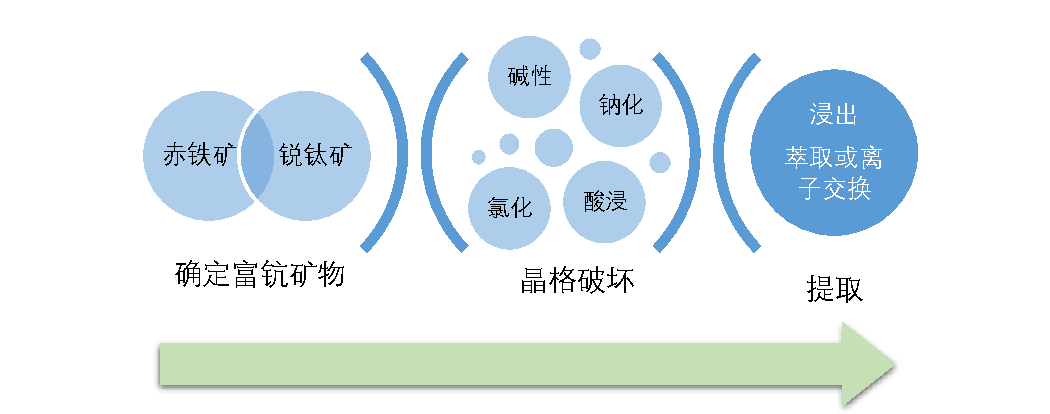
\includegraphics[width=\linewidth]{Figures/c1/technicalroute.pdf}%width=0.7大概为原来的100%。
	%\hspace{2pt}\includegraphics[width=0.45\linewidth]{Figures/Fig2}%\hspace设置水平间距
	\caption{课题研究思路}\label{technicalroute}
\end{figure}
\section{论文主要研究内容}

论文的研究内容主要包括以下几个方面:

(1) 多金属赤泥基本物化性质

主要是钪与主元素铁、铝、硅、钛、钙的亲和行为。

(2) 赤泥中钠的预分离探究

主要是不同冷却方式对活化焙烧赤泥中钠的预分离以及物相种类和结构的影响规律。

(3) 赤泥硫酸化焙烧与钪选择性浸出机理

a) 硫酸盐焙烧相变机理研究;

b) 硫酸盐化赤泥焙烧后Sc、Na、Fe、Al、Ti、Ga、Ca和Si的浸出行为;

(4) 硫酸盐化焙烧后赤泥浸出液中钪钠分离

主要是硫酸盐化焙烧赤泥浸出液中钪的溶剂萃取参数确定。


\nomenclature{DSP}{Desilication products脱硅产物}